\documentclass[11pt,a4paper]{article}

% ── Packages ──────────────────────────────────────────────────────────────────
\usepackage[T1]{fontenc}
\usepackage[utf8]{inputenc}
\usepackage{lmodern}
\usepackage[margin=2.5cm]{geometry}
\usepackage{amsmath,amssymb,amsthm}
\usepackage{booktabs}
\usepackage{array}
\usepackage{graphicx}
\usepackage[labelfont=bf,font=small,skip=4pt]{caption}
\usepackage{subcaption}
\usepackage{float}
\usepackage{xcolor}
\usepackage[colorlinks=true,linkcolor=blue!60!black,citecolor=green!50!black,
            urlcolor=blue!70!black]{hyperref}
\usepackage{microtype}
\usepackage{parskip}
\usepackage{enumitem}
\usepackage{fancyhdr}
\usepackage[numbers,sort&compress]{natbib}

\graphicspath{{figures/}}
\captionsetup{font=normalsize,labelfont=bf,skip=6pt}
\captionsetup[sub]{font=small,skip=3pt}

\pagestyle{fancy}
\fancyhf{}
\rhead{\small Spectral filters for track finding}
\lhead{\small G.\,W.\,Scriven}
\cfoot{\thepage}
\renewcommand{\headrulewidth}{0.4pt}

\newtheorem{theorem}{Theorem}
\newcommand{\eff}{\ensuremath{\varepsilon_{\rm seg}}}
\newcommand{\far}{\ensuremath{f_{\rm seg}}}

% ── Title ─────────────────────────────────────────────────────────────────────
\title{From one bit to a fitted polynomial:\\
engineered spectral filters for track reconstruction\\
in a noisy LHCb VELO toy model}

\author{George William Scriven\thanks{george.w.scriven@gmail.com}\\[2pt]
\normalsize Maastricht University, Maastricht, The Netherlands\\
\normalsize Hasselt University, Hasselt, Belgium\\
\normalsize Nikhef, Amsterdam, The Netherlands}

\date{\today}

\begin{document}
\maketitle

\begin{abstract}
Track reconstruction in the LHCb vertex detector can be written as a linear
system $A\mathbf{x}=\mathbf{b}$ over track \emph{segments}, whose solution
scores each segment by how strongly its neighbours reinforce it. Two earlier
papers solved this system with quantum linear algebra: first with the HHL
algorithm, and then far more cheaply with a one-bit variant, the one-bit
quantum filter (1BQF), which replaces the full inversion by a single cosine
filter of the Hamiltonian with one spectral zero. In this paper I develop
that idea further. The 1BQF is the degree-one member of the family of
polynomial spectral transforms provided by the quantum singular value
transformation (QSVT), and once the problem is viewed this way the design
question changes: it is no longer a question of which algorithm inverts
$A$, but of which function of $\lambda$ separates true from false segments.
On clean events the answer is a four-line comb pinned to the eigenvalues of
a five-hit track, and it drives the segment false rate from $20.5\%$
(classical, $T{=}1000$ tracks) to $0.9\%$ at $92\%$ efficiency. On noisy
events the answer must be measured: the false weight piles up on the
eigenvalue lines of specific two- and three-segment motifs, and a
polynomial fitted with roots at the measured pile-up beats the classical
baseline at every attainable efficiency below a sharply defined
\emph{fragment floor}, the small population of true fragments that are
spectral twins of the false motifs and that, on that Hamiltonian, no
function of $\lambda$ can separate. I also show that the two natural Hamiltonian modifications
inherited from the classical literature can only be judged together with
the response applied to them. The Denby--Peterson occupancy term destroys
the one-bit filter, whose single zero cannot follow the spectrum it
creates; but paired with a response refitted to that spectrum it becomes
the strongest configuration in the study, roughly halving the fitted
false rate at every matched efficiency, and, at small coupling, it breaks
the spectral-twin degeneracy behind the fragment floor: the floor is a
property of the base Hamiltonian, not of the problem. The bifurcation
(fork) term behaves the same way, a regression under the clean-event comb
and a net win under the refitted response. The result is a two-part
design rule: the operator shapes the spectrum, and the fitted response
separates it; neither knob can be evaluated without the other.
\end{abstract}

% ══════════════════════════════════════════════════════════════════════════════
\section{Introduction}
\label{sec:intro}

Charged-particle track reconstruction is, at heart, a combinatorial
matching problem: a detector hands us a cloud of hits, and we must decide
which hits belong together. At the High-Luminosity LHC this cloud becomes
dense enough that the matching cost dominates real-time reconstruction
budgets, and the tracking community has responded by testing essentially
every alternative computing platform: GPUs, FPGAs, neural networks, and, in
the line of work this paper continues, quantum computers.

The lineage of this work is short and worth stating precisely. Nicotra et
al.~\cite{nicotra2023} showed that track reconstruction in a simplified
model of the LHCb vertex detector (VELO) can be phrased as a linear system
$A\mathbf{x}=\mathbf{b}$ over track segments and solved with the
Harrow--Hassidim--Lloyd algorithm~\cite{hhl2009}; a restricted-phase-estimation
variant of that construction was subsequently reported in
ref.~\cite{trackhhl_epj}. The follow-up
paper~\cite{trackhhl} observed that the full inversion is overkill. The
interesting information is which segments are active, not their precise
weights, so a single-ancilla circuit, the one-bit quantum filter (1BQF),
suffices. The 1BQF applies one cosine function of the Hamiltonian, placed
so that its zero lands exactly on the eigenvalue shared by every isolated
fake segment, and reads out the survivors. It is cheap, it suits near-term
hardware, and it was demonstrated on trapped-ion and superconducting
devices.

This paper asks the question that follows naturally from the 1BQF. A
cosine with one zero is a polynomial filter of degree
one\footnote{Strictly, a trigonometric function realised at degree one in
the Chebyshev basis of the walk operator; section~\ref{sec:qsvt} makes
this exact.}. The quantum singular value transformation
(QSVT)~\cite{gslw2019,martyn2021} tells us that a quantum computer can
apply essentially any bounded polynomial of the Hamiltonian at a cost
linear in its degree. So, what could we do with more than one zero? Which
polynomial should we choose? And what happens to that choice when the
Hamiltonian itself changes, because the detector is noisy or because we
have added constraint terms to help it? In my opinion this last question
carries most of the physics, and most of this paper is spent answering
it.

I answer these questions on the same toy model as the two predecessor
papers, extended with realistic noise. The answers can be summarised as a
single working method, which I will refer to as fitting the response to
the spectrum:

\begin{enumerate}[leftmargin=2em]
\item On clean events the true-track spectrum is \emph{discrete}: detector
geometry pins every true track to the same five-hit chain, whose four
eigenvalues are known in closed form. A comb of narrow passes at those
four lines, and nothing else, separates true from false essentially
perfectly up to the densities I can simulate ($T=1000$ tracks, four
million segments), where the classical solver's false rate has climbed to
$20.5\%$.
\item On noisy events the false population moves: it concentrates on the
eigenvalue lines of specific small \emph{motifs} (hit-sharing pairs and
triples), which sit off the true lines but inside any naive pass window.
The correct response cannot be written down a priori; it must be fitted
to the measured pile-up. Once it is, the quantum false rate drops below
the classical one at every efficiency below a floor that I can identify,
count, and explain segment by segment.
\item Hamiltonian engineering and response engineering are coupled, and
neither knob can be evaluated without the other. Both Denby--Peterson
penalties destroy the one-bit filter and read as regressions under the
fixed clean-event comb; both become net wins once the polynomial is
refitted to the spectrum they produce. The occupancy term is the
sharpest case: it breaks the notch outright, yet with a refitted
response it roughly halves the false rate at every matched efficiency,
and at small coupling it lifts the fragment floor by breaking the
spectral-twin degeneracy that causes it. Changing the operator moves
the activations, and moving the activations changes the polynomial we
have to fit.
\end{enumerate}

The paper is organised as follows. Section~\ref{sec:toy} builds the toy
model and the segment Hamiltonian from zero, including the exact
activation levels that make everything else quantitative.
Section~\ref{sec:onebit} reviews the 1BQF as a spectral filter and
establishes the working-point conventions used throughout.
Section~\ref{sec:qsvt} develops the QSVT machinery (block encoding,
qubitization, and the linear-combination-of-Chebyshev construction) at
the level of detail needed to count qubits and gates.
Section~\ref{sec:comb} designs and evaluates the line comb on clean
events, including its resource scaling and its provable limits.
Section~\ref{sec:noise} introduces the noise model and shows what it does
to each solver. Section~\ref{sec:occupancy} dissects the occupancy
term's collision with the notch. Section~\ref{sec:fork} introduces the
fork term and the design rule that every operator change demands a
response refit. Section~\ref{sec:fit} fits the polynomial to the
measured false pile-up and presents the main comparison, including the
refitted occupancy result. Section~\ref{sec:limits}
collects the limitations: realizability, the single-response question,
Trotterization,
and what a real detector geometry changes. Section~\ref{sec:conclusion}
concludes.

A remark on style before we begin. This paper is deliberately verbose.
The predecessor papers compressed the segment-Hamiltonian formalism to a
few paragraphs; here I want every level, every eigenvalue, and every
convention on the table, because the physics of why filters succeed and
fail lives in exactly those details.

% ══════════════════════════════════════════════════════════════════════════════
\section{The toy model and the segment Hamiltonian}
\label{sec:toy}

\subsection{Events}
\label{sec:toy:events}

The toy detector is the standard simplified VELO of
refs.~\cite{nicotra2023,trackhhl}: parallel planes perpendicular to the
beam axis ($z$), each recording a two-dimensional point where a charged
particle crosses it. An event is generated by drawing $T$ tracks from a
common primary vertex on the $z$-axis, with polar angles inside a
generation cone, and propagating each as a straight line through the
planes. Every track leaves one hit per plane. Detector effects enter as
controlled perturbations, and I will always state the triple in force:
multiple-scattering kinks of width $\sigma_{\rm scatt}$ applied at each
plane crossing, Gaussian hit-position smearing of width
$\sigma_{\rm res}$, and a hit-drop (inefficiency) probability applied hit
by hit. The clean configuration used in section~\ref{sec:comb} is
$(\sigma_{\rm scatt},\sigma_{\rm res},{\rm drop})=(10^{-4},\,0,\,0)$; the
heavy configuration used from section~\ref{sec:noise} onward is
$(10^{-4},\,20\,\mu\mathrm{m},\,1\%)$.

A \emph{segment} is an ordered pair of hits on adjacent planes. With five
planes and $T$ hits per plane, each of the four inter-plane gaps offers
$T^2$ candidate segments, so
\begin{equation}
n_{\rm seg}=4T^{2},\qquad n_{\rm true}=4T,\qquad
n_{\rm false}=4T(T-1),
\label{eq:combinatorics}
\end{equation}
where $n_{\rm true}$ counts the segments that connect two hits of the
same generated track. The problem is a needle in a haystack, and the
ratio $n_{\rm true}/n_{\rm seg}=1/T$ says how deep the hay is: at
$T=1000$ only one segment in a thousand is real, and the false population
grows quadratically while the true one grows linearly. Any segment
classifier, classical or quantum, fights this composition before it
fights anything else.

\subsection{The Hamiltonian}
\label{sec:toy:ham}

Following Denby and Peterson's neural formulation of track
finding~\cite{denby1988,peterson1989} as adapted by
refs.~\cite{nicotra2023,trackhhl}, we encode an event in a quadratic
energy over segment activations $x_i\in\mathbb{R}$,
\begin{equation}
E(\mathbf{x})=\tfrac12\,\mathbf{x}^{\!\top}\!A\,\mathbf{x}
-\delta\,\mathbf{1}^{\!\top}\mathbf{x},
\qquad
A=(\gamma+\delta)\,I-C,
\label{eq:energy}
\end{equation}
where $C$ is the 0/1 \emph{compatibility adjacency}: $C_{ij}=1$ exactly
when segments $i$ and $j$ share a hit as head-to-tail continuations (the
end hit of one is the start hit of the other) and their mutual angle is
below an acceptance $\varepsilon$. The constants are a self-penalty
$\gamma$ (discouraging indiscriminate activation) and a bias $\delta$
(rewarding activation); throughout the main text $\gamma=3$, $\delta=1$,
so the constant diagonal is $s\equiv\gamma+\delta=4$. Minimising
eq.~\eqref{eq:energy} gives the linear system
\begin{equation}
A\,\mathbf{x}=\delta\,\mathbf{1},
\label{eq:linsys}
\end{equation}
which I solve classically with MINRES ($A$ is symmetric, sparse, and at
$\gamma=3$ comfortably positive definite). A useful picture is a voting
market: each segment starts with the same bias-funded credit $\delta$,
and the off-diagonal couplings let aligned neighbours reinforce one
another. A segment embedded in a long, straight chain of compatible
neighbours accumulates support; a segment with no compatible continuation
is left with only its own bias against its own penalty.

The acceptance $\varepsilon$ deserves its own paragraph, because it is
the single most consequential experimental knob. It is set by a
closed-form formula from the expected root-mean-square kink between
consecutive true segments under the noise triple in force, with a
$3\sigma$ margin so that true continuations pass the angular cut:
\begin{equation}
\varepsilon=\sqrt{\,2\,(3\sigma_{\rm scatt})^{2}
+12\,\arctan^{2}\!\big(3\sigma_{\rm res}/\Delta z\big)
+2\,\theta_{\min}^{2}\,},
\label{eq:epsilon}
\end{equation}
where $\Delta z=33$\,mm is the inter-plane spacing, the first term
budgets the multiple-scattering kink between the two segments, the
second the angle that hit-position smearing subtends across one plane
gap, and $\theta_{\min}=15\,\mu$rad is a numerical floor for the
noise-free limit. On the heavy configuration
eq.~\eqref{eq:epsilon} gives $\varepsilon=6.3\,$mrad, fifteen times
wider than the clean-configuration value, and section~\ref{sec:noise}
shows what that width admits.

\subsection{Exact activation levels: the atlas}
\label{sec:toy:levels}

Because $A$ has constant diagonal, its action decomposes over the
connected components of the compatibility graph, and small components can
be solved by hand. This is worth doing once in full, because these little
closed forms are the vocabulary of every result in the paper.

An \emph{isolated} segment (no compatible neighbour) has the scalar
equation $(\gamma+\delta)x=\delta$, so
\begin{equation}
x_{\rm iso}=\frac{\delta}{\gamma+\delta}=\frac14=0.250 .
\label{eq:iso}
\end{equation}
This is the false \emph{attractor}: at any multiplicity, the
overwhelming majority of the $4T(T-1)$ false segments are isolated and
sit at exactly $0.250$. A true track, by contrast, is a path $P_4$ of
four segments (five hits), whose matrix is $sI-P_4$ with $P_4$ the path
adjacency. Its solution can be written down exactly:
\begin{equation}
x_{\rm outer}=\frac{4}{11}\approx0.364,\qquad
x_{\rm inner}=\frac{5}{11}\approx0.455 ,
\label{eq:p4levels}
\end{equation}
where the outer levels belong to the two end segments (one continuation
neighbour each) and the inner levels to the two middle segments (two
neighbours each).

These numbers, and the whole family behind them, come from one small
calculation that is worth doing explicitly. A chain of $m$ segments
has the matrix $sI-P_m$ with $P_m$ the path adjacency, so the $j$-th
row of $(sI-P_m)\,\mathbf{x}=\delta\mathbf{1}$ reads
\[
-x_{j-1}+s\,x_j-x_{j+1}=\delta ,\qquad j=1,\dots,m ,
\]
a three-term linear recurrence, provided we adopt the convention
$x_0=x_{m+1}=0$: an end segment simply has no neighbour on one side,
which is the same as coupling it to a phantom segment clamped at
zero. A recurrence of this kind is solved by any particular solution
plus the general homogeneous one. The natural particular solution is
the constant
\[
\bar x=\frac{\delta}{s-2}=\frac12 \qquad (s=4,\ \delta=1),
\]
the activation of a segment deep inside an infinitely long chain,
where both neighbours carry the same value and the row equation
collapses to $(s-2)\,\bar x=\delta$. The homogeneous solutions of
$-x_{j-1}+s\,x_j-x_{j+1}=0$ are the geometric sequences $r^{\,j}$
with
\[
r+\frac{1}{r}=s
\quad\Longrightarrow\quad
r=\frac{s-\sqrt{s^{2}-4}}{2}=2-\sqrt3\approx0.268 ,
\]
a decaying root and its growing mirror $1/r$. Writing the general
solution as $x_j=\bar x+A\,r^{\,j}+B\,r^{\,m+1-j}$ (one geometric
correction anchored at each end) and imposing the two clamped-end
conditions $x_0=x_{m+1}=0$ forces, by the chain's reflection
symmetry, $A=B=-1/\big(2\,(1+r^{m+1})\big)$, so the entire
activation profile has the closed form
\[
x_j=\frac12-\frac{r^{\,j}+r^{\,m+1-j}}{2\,(1+r^{m+1})} .
\]
The picture behind the algebra: each end of the chain is a cold
boundary that drags the activation below the bulk value $\tfrac12$
by a deficit decaying geometrically into the interior, with
penetration depth $1/\ln(1/r)\approx0.76$ segments. Setting $j=1$
(or, identically, $j=m$) gives the outer activation
\begin{equation}
x_{\rm outer}(m)=\frac12-\frac{r+r^{m}}{2\,(1+r^{m+1})},
\qquad r=2-\sqrt3,
\label{eq:ladder}
\end{equation}
and $j=2$ at $m=4$ returns the inner $5/11$ of
eq.~\eqref{eq:p4levels}. Equation~\eqref{eq:ladder} climbs the ladder
$\{0.250,\ \tfrac13,\ \tfrac{5}{14},\
\tfrac{4}{11},\dots\}\nearrow(1-r)/2=(\sqrt3-1)/2\approx0.366$ for
$m=1,2,3,4,\dots$: a short chain sits low because the two boundary
deficits overlap, and the ladder saturates once the ends are further
apart than the penetration depth. It is worth
working two rungs by hand. A two-hit fragment ($m{=}1$) sits at exactly
the isolated-false attractor $0.250$, and a three-hit fragment ($m{=}2$)
sits at $1/3$, only $0.083$ above it. Fragments are barely
distinguishable from noise by amplitude alone; this innocent-looking
fact returns as the fragment floor in section~\ref{sec:fit}.

\begin{figure}[t]
\centering
\captionsetup{width=0.85\textwidth}
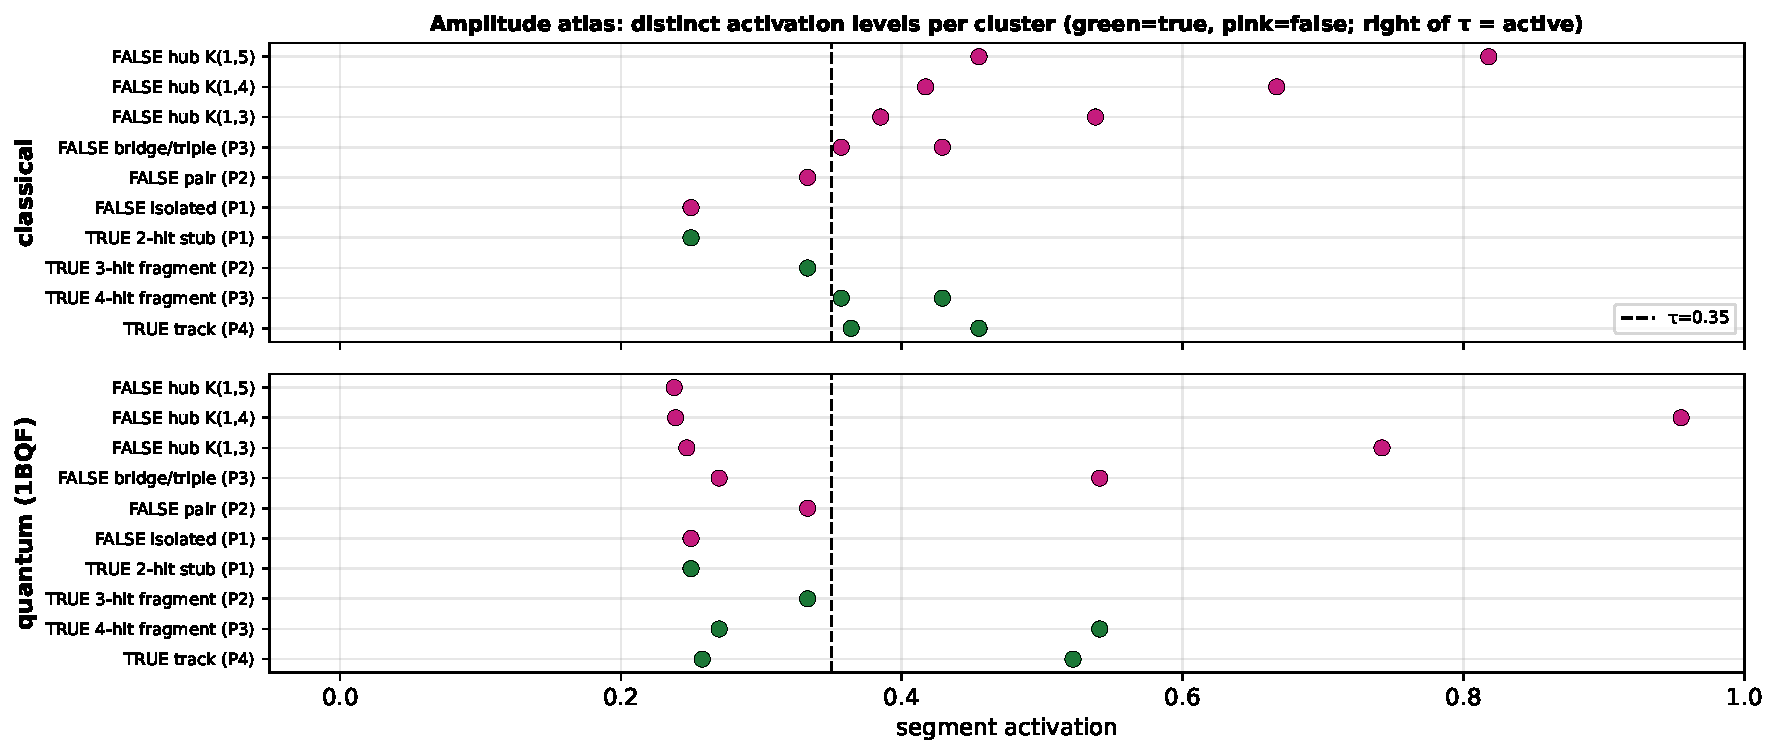
\includegraphics[width=0.9\textwidth]{amplitude_atlas.pdf}
\caption{The amplitude atlas: exact activation level of every canonical
cluster type (rows), classical (top) and 1BQF-filtered (bottom), with the
fixed threshold $\tau=0.35$ marked. Green: true; pink: false. Everything
quantitative in this paper is a statement about where these levels sit
relative to a threshold.}
\label{fig:atlas}
\end{figure}

The classical decision rule is a threshold: segment $i$ is \emph{active}
iff $x_i>\tau$. The \emph{classical} convention, inherited from
ref.~\cite{trackhhl} and kept for comparability, fixes
\begin{equation}
\tau(\gamma,\delta)=\frac{\delta}{\gamma+\delta}+0.10 ,
\label{eq:tau}
\end{equation}
i.e.\ $\tau=0.35$ at $\gamma=3$: a fixed margin above the false
attractor, below the lowest clean-track level $4/11$. It is important
to say at the outset what this convention is and is not. For the
classical solver it is a natural operating point, because the classical
amplitude atlas happens to leave a gap there. For a \emph{filtered}
solver it is in general the wrong place to read the device: a filter
reshapes the amplitude atlas, and a threshold inherited from the
unfiltered atlas can land in the middle of a reshaped true band.
Every threshold choice trades efficiency against false rate, and the
convention this paper actually uses for filtered solvers is
\emph{efficiency-first}: put the threshold where the wanted fraction of
true segments survives, and quote the false rate that results.
Section~\ref{sec:onebit} makes this concrete, with the trade-off shown
explicitly in figure~\ref{fig:threshold}.

\subsection{Metric definitions}
\label{sec:toy:metrics}

Every number in this paper is one of the following, and I will never use
these words in any other sense:
\begin{itemize}[leftmargin=2em]
\item \textbf{segment efficiency} $\eff=n_{\rm true\,active}/n_{\rm true}$:
the fraction of true segments that survive selection;
\item \textbf{segment false rate}
$\far=n_{\rm false\,active}/n_{\rm active}$: the fraction of the
\emph{selected} sample that is fake (note the denominator: this is an
impurity, not a false-positive rate over all fakes);
\item \textbf{working points}: either the \emph{fixed threshold} of
eq.~\eqref{eq:tau}; or the \emph{efficiency-first working point}
(the threshold placed just below the 1\% quantile of the true-segment
amplitudes, so $\eff\ge0.99$ by construction --- whenever this paper
says ``efficiency-first'' without qualification, this 99\% point is
meant); or, in
sections~\ref{sec:fork}--\ref{sec:fit}, the \emph{matched-efficiency}
convention: $\tau$ just below the $k$-th largest true amplitude with
$k=\lceil\mathrm{eff}\cdot n_{\rm true}\rceil$, which lets solvers be
compared at identical efficiency without quantile-grid artefacts.
\item \textbf{AUC}, the threshold-free separation metric: sweeping
$\tau$ from high to low traces out a curve of efficiency against false
rate for each solver, and the \emph{area under that curve} summarises
how well the solver's amplitude ordering separates true from false
segments independently of any particular threshold choice. AUC~$=1$
means some threshold separates them perfectly; AUC~$=0.5$ means the
ordering is no better than chance. It is used when a single number for
``separation quality'' is needed, notably in
section~\ref{sec:occupancy}.
\end{itemize}
Quantum solutions are unit-norm vectors; before thresholding they are
rescaled to the classical amplitude scale on the classically-active
support. Rescaling by the full norm would be multiplicity-dependent,
since the false bulk owns most of the norm, and was the source of a
metric artefact documented in the programme's earlier write-ups. All
thresholds act on $|x_i|$.

\subsection{The spectrum}
\label{sec:toy:spectrum}

Because $A=sI-C$, its spectrum is a rigid reflection of the
compatibility graph's: $\lambda(A)=s-\mu(C)$, where $\mu(C)$ denotes an
eigenvalue of $C$, the $\varepsilon$-windowed 0/1 compatibility
adjacency of section~\ref{sec:toy:ham} ($C_{ij}=1$ exactly when
segments $i$ and $j$ continue one another head-to-tail within the
angular acceptance $\varepsilon$, and $0$ otherwise). Every spectral
statement in this paper is therefore a statement about the eigenvalues
of small 0/1 graphs. Three families matter:
\begin{enumerate}[leftmargin=2em]
\item \textbf{Isolated segments}: $\lambda=s$ exactly. This single line
carries $\mathcal{O}(n_{\rm seg})$ modes: at $T=200$ under heavy noise,
$155{,}371$ of $157{,}609$ segments (rep~0).
\item \textbf{Chains} $P_m$: $\lambda_k=s-2\cos\!\big(k\pi/(m{+}1)\big)$,
$k=1,\dots,m$. A true track ($m=4$) therefore lives on exactly four
lines,
\begin{equation}
\lambda\in\{s-2\cos(k\pi/5)\}_{k=1}^{4}
=\{2.382,\ 3.382,\ 4.618,\ 5.618\}\quad(s=4),
\label{eq:p4lines}
\end{equation}
symmetric about $s$ and split by the golden-ratio
cosines\footnote{The values $2\cos(\pi/5)=\varphi=1.618\dots$ and
$2\cos(2\pi/5)=1/\varphi$: the five-hit track is secretly a pentagon
problem.}.
\item \textbf{Stars} $K_{1,m}$ (one hit shared by $m$ segments of the
same role): $\lambda=s\pm\sqrt m$ plus $m{-}1$ copies of $s$.
\end{enumerate}
Figure~\ref{fig:motifs} draws each of these motifs in hit space and
places its exact eigenvalue lines on a common $\lambda$-axis: this is
the dictionary between what a cluster of segments \emph{looks like} in
the detector and where its solution weight \emph{piles up} in the
spectrum. The pair motif at $\lambda=s\pm1$ and the triple at
$\{s,\,s\pm\sqrt2\}$ do most of the false-population work under noise,
and their lines interleave the true lines of eq.~\eqref{eq:p4lines}
without touching them. That gap, false lines close to but not on the
true lines, is what this paper exploits. When noise is switched on in
section~\ref{sec:noise}, the \emph{measured} spectral pile-up of a
heavy-noise event (figure~\ref{fig:pileup}) lands exactly on the lines
catalogued here. Motifs whose spectrum coincides
with a true motif's are the exception, and they return in
sections~\ref{sec:comb:limits} and~\ref{sec:fit} as the limiting factor.

\begin{figure}[t]
\centering
\captionsetup{width=0.95\textwidth}
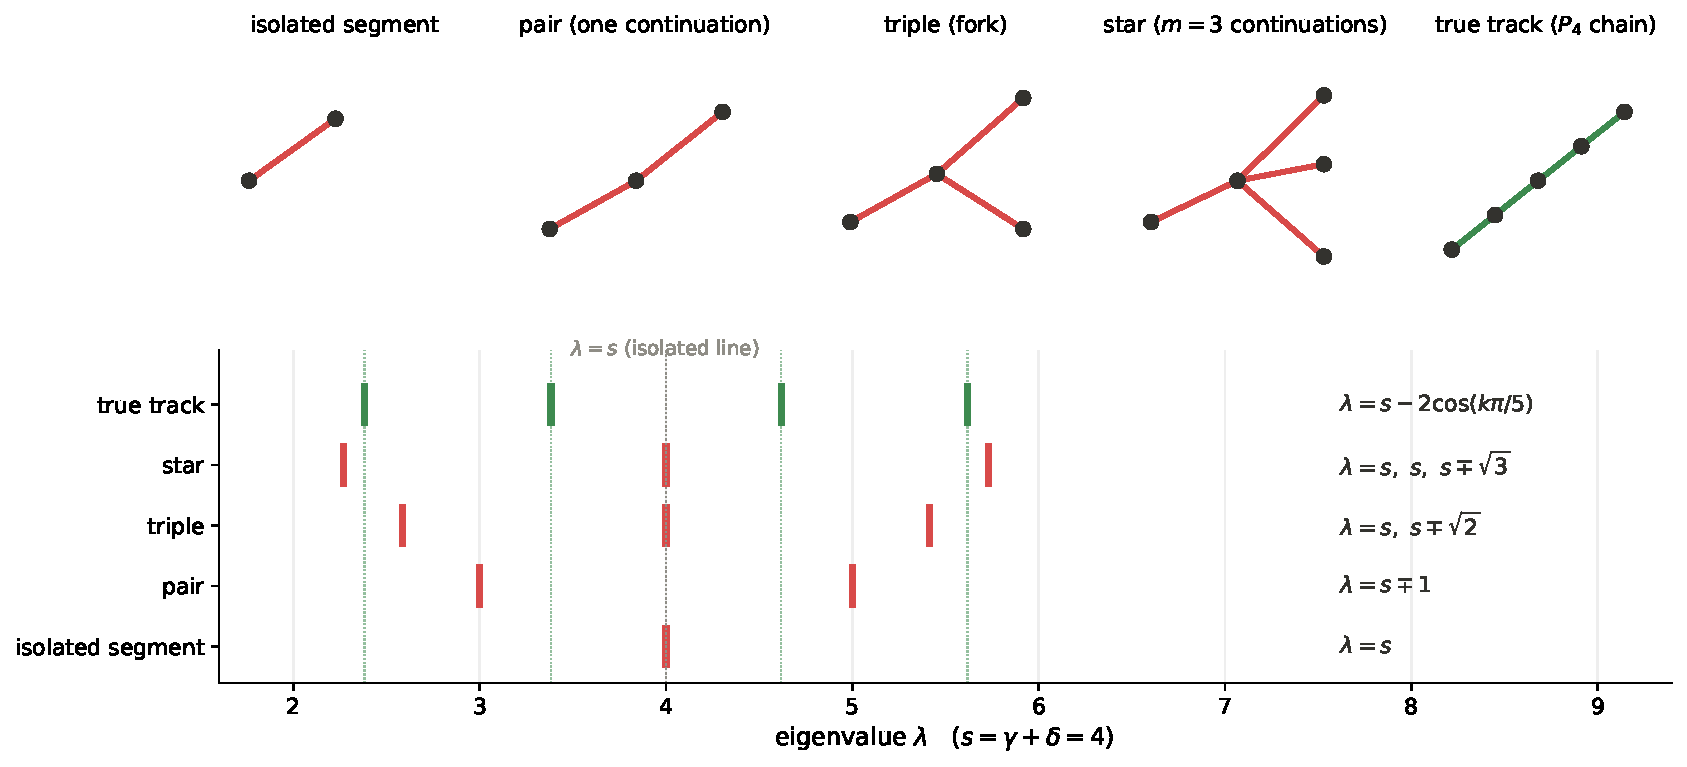
\includegraphics[width=0.98\textwidth]{motif_gallery.pdf}
\caption{The motif dictionary. Top: the canonical segment clusters
drawn in hit space (dots are hits, lines are segments; green true, red
false). Bottom: the exact eigenvalue lines each motif contributes,
from the closed forms of section~\ref{sec:toy:spectrum}, at
$s=\gamma+\delta=4$. Every false family sits close to, but never on,
the four true-track lines (green dotted) --- except for the spectral
twins of section~\ref{sec:comb:limits}.}
\label{fig:motifs}
\end{figure}

% ══════════════════════════════════════════════════════════════════════════════
\section{The one-bit quantum filter, read as a spectral filter}
\label{sec:onebit}

\subsection{The circuit and its response function}

The 1BQF of ref.~\cite{trackhhl} is a one-ancilla interference
experiment. Prepare the uniform superposition $|u\rangle$ over the
(zero-padded) segment register, put the ancilla in
$(|0\rangle+|1\rangle)/\sqrt2$, apply $e^{iAt}$ to the register
controlled on the ancilla, close the interferometer with a second
Hadamard, and keep the runs in which the ancilla reports the
interference branch. The kept state is
\begin{equation}
|\psi\rangle \;\propto\; \tfrac12\big(I+e^{iAt}\big)|u\rangle
\;=\;\sum_i e^{i\lambda_i t/2}\cos\!\Big(\frac{\lambda_i t}{2}\Big)\,
\langle v_i|u\rangle\,|v_i\rangle ,
\label{eq:onebitresponse}
\end{equation}
where $\{\lambda_i,|v_i\rangle\}$ are the eigenpairs of $A$. Reading
out $|\langle j|\psi\rangle|$ segment by segment gives amplitudes
$x^{Q}_j$, and the whole device is summarised by a single real
response function applied to the spectrum:
\begin{equation}
f(\lambda)=\cos\!\Big(\frac{\lambda t}{2}\Big),
\qquad t=\frac{\pi}{s} .
\label{eq:notch}
\end{equation}
The choice $t=\pi/s$ places the zero of the cosine exactly at
$\lambda=s$, the isolated-segment line. Every isolated false segment,
all $\mathcal{O}(n_{\rm seg})$ of them, is annihilated exactly: not
suppressed, killed. This is the entire content of the 1BQF, and the
form in which we will need it later is a simple accounting rule: each
application of the filter buys exactly one zero of the response, and
the 1BQF spends its one zero on the largest false population in the
problem. The padding modes introduced to reach a power-of-two
dimension are diagonal-only, sit at $\lambda=s$ too, and are removed
by the same zero, a small but pleasing piece of engineering hygiene.

Figure~\ref{fig:responses} makes the geometry of this choice, and of
everything that follows, visible. The top panel is the 1BQF response
of eq.~\eqref{eq:notch} drawn over the populated spectrum: its single
zero sits exactly on the isolated-false line, and every other
population, the pair and triple motif lines included, lands on the
slopes of the cosine and passes with large weight. The filter attacks
the isolated segments and nothing else; whatever false weight is
\emph{coupled} sails through. The bottom panel shows the QSVT
alternative developed from section~\ref{sec:qsvt} onward: a degree-40
polynomial with narrow passes at the four true-track lines and
effective zeros everywhere else, including the isolated, pair and
triple lines simultaneously. The one-sentence summary of this paper
is the difference between those two panels: a degree-one response owns
one zero, a degree-$d$ response owns $d$, and the noisy-event false
spectrum demands more than one.

\begin{figure}[t]
\centering
\captionsetup{width=0.90\textwidth}
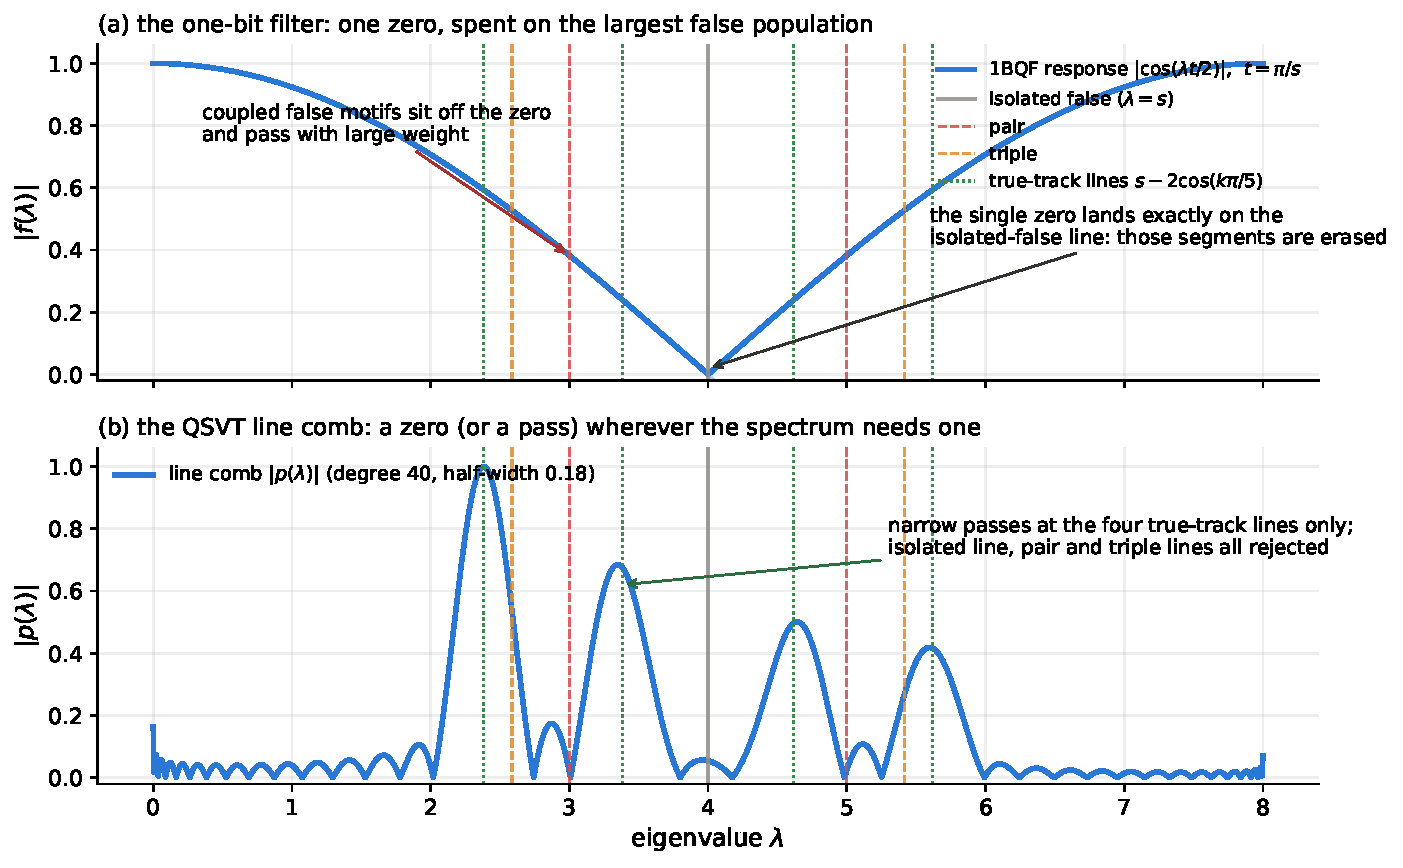
\includegraphics[width=0.92\textwidth]{response_functions.pdf}
\caption{The two response functions against the populated spectrum
($s=4$). (a) The 1BQF cosine: one zero, placed on the isolated-false
line; the coupled false motifs (pair, triple) sit on the slopes and
pass. (b) The degree-40 line comb: passes at the four true-track
lines only, with the isolated, pair and triple lines all rejected.}
\label{fig:responses}
\end{figure}

\subsection{What the notch cannot do}

Away from its zero the cosine is not flat, and this has two
consequences that define the 1BQF's operating envelope.

The first is that true amplitudes are reshaped. A true track's four
modes (eq.~\eqref{eq:p4lines}) sit symmetrically about $s$, where
$|f(\lambda)|$ is small; the filtered chain no longer reproduces the
classical $\{4/11,5/11\}$ profile. The effect has a closed form: the
outer (endpoint) segments of a clean track drop from $0.364$ to
$0.258$, below the fixed threshold $\tau=0.35$, while the inner pair
survives above it. At the fixed threshold the 1BQF therefore reports a
segment efficiency plateau of $\approx0.73$--$0.75$: it finds the
middles of tracks and loses the ends. This endpoint loss is a
property of the cut, not of the physics; the endpoint amplitudes
remain perfectly well ordered above the false ones, so a threshold
placed below the endpoint band recovers them all.

Figure~\ref{fig:threshold} shows the whole trade explicitly, on a
stored $T=400$ clean event, by sweeping the threshold for all three
solvers of this paper. The efficiency panel shows the plateau
structure just described: the 1BQF efficiency steps down at the
endpoint band around $\tau\approx0.28$, so the inherited $\tau=0.35$
reads $75\%$ --- not because the filter lost the physics but because
the cut sits above a reshaped true band. The false-rate panel shows
what moving the threshold costs. Every solver is therefore read at
its own \emph{efficiency-first working point} (dashed verticals):
the threshold just below the 1\% quantile of that solver's true
amplitudes, so that $99\%$ of true segments survive by construction,
with the false rate quoted as the price. This is the convention for
all 1BQF headlines in this paper; the fixed $\tau=0.35$ of
eq.~\eqref{eq:tau} is retained only where the classical baseline is
quoted on its own established operating point. On clean
fixed-acceptance events at $\gamma=3$ the efficiency-first price is
steep at high multiplicity: the 1BQF false rate climbs to several
tens of percent by $T=400$ and beyond, and section~\ref{sec:comb}
quantifies this against the comb.

\begin{figure}[t]
\centering
\captionsetup{width=0.92\textwidth}
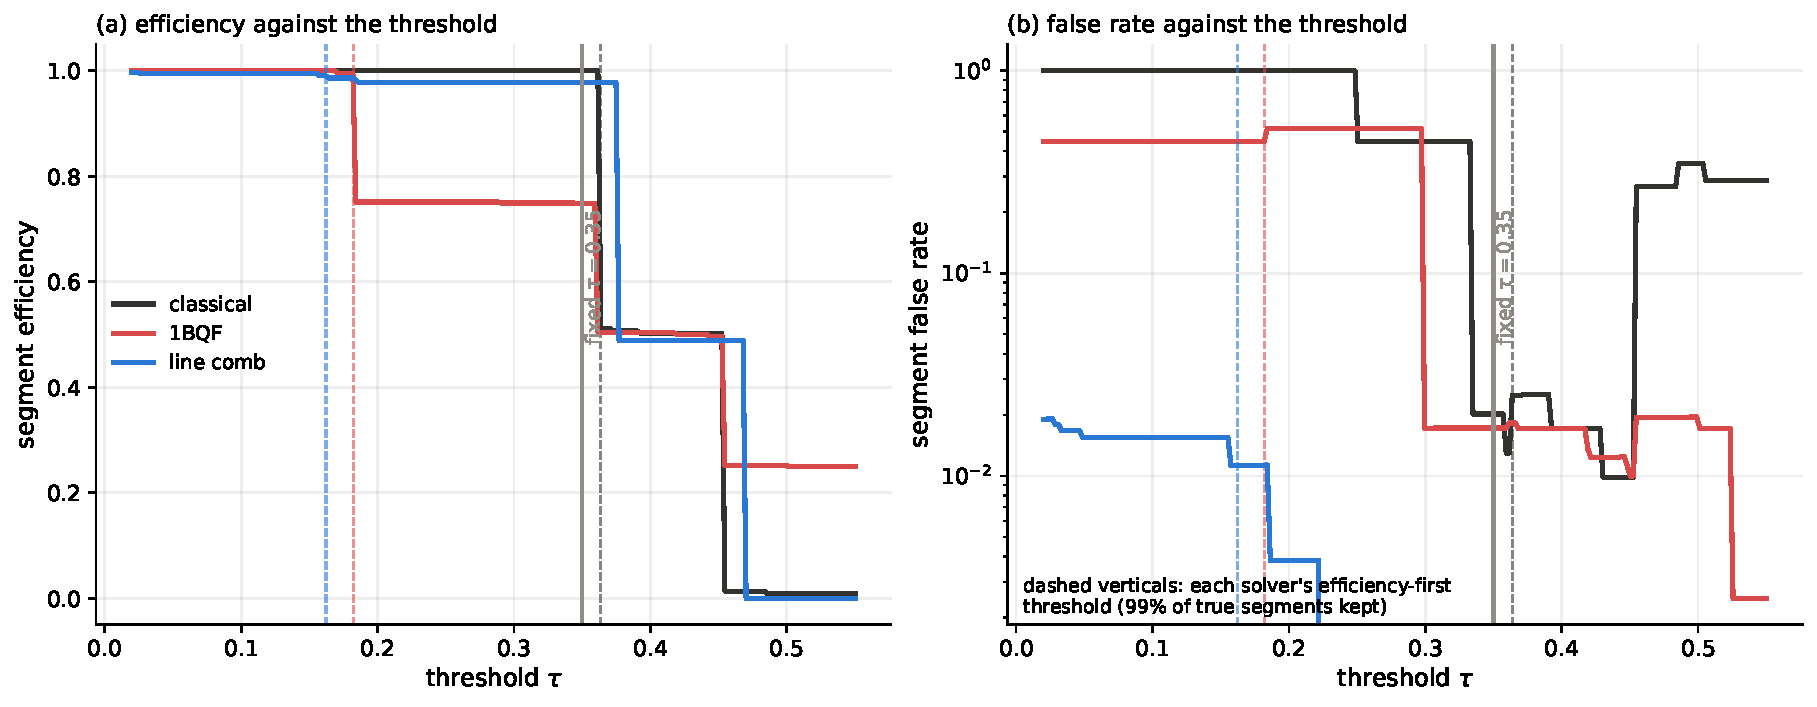
\includegraphics[width=0.95\textwidth]{threshold_tradeoff.pdf}
\caption{The threshold trade-off, on the stored $T=400$ clean event of
the canonical campaign: (a) segment efficiency and (b) segment false
rate as the threshold $\tau$ sweeps, for the classical solver, the
1BQF and the line comb (quantum amplitudes on the classical signal
scale). The grey vertical is the inherited fixed $\tau=0.35$; the
dashed verticals are each solver's efficiency-first working point
(99\% of its true segments kept). The fixed cut sits above the 1BQF's
reshaped endpoint band --- the origin of its $75\%$ plateau --- while
the comb holds both high efficiency and a $\sim10^{-2}$ false rate
over the whole usable range.}
\label{fig:threshold}
\end{figure}

\begin{figure}[t]
\centering
\captionsetup{width=0.70\textwidth}
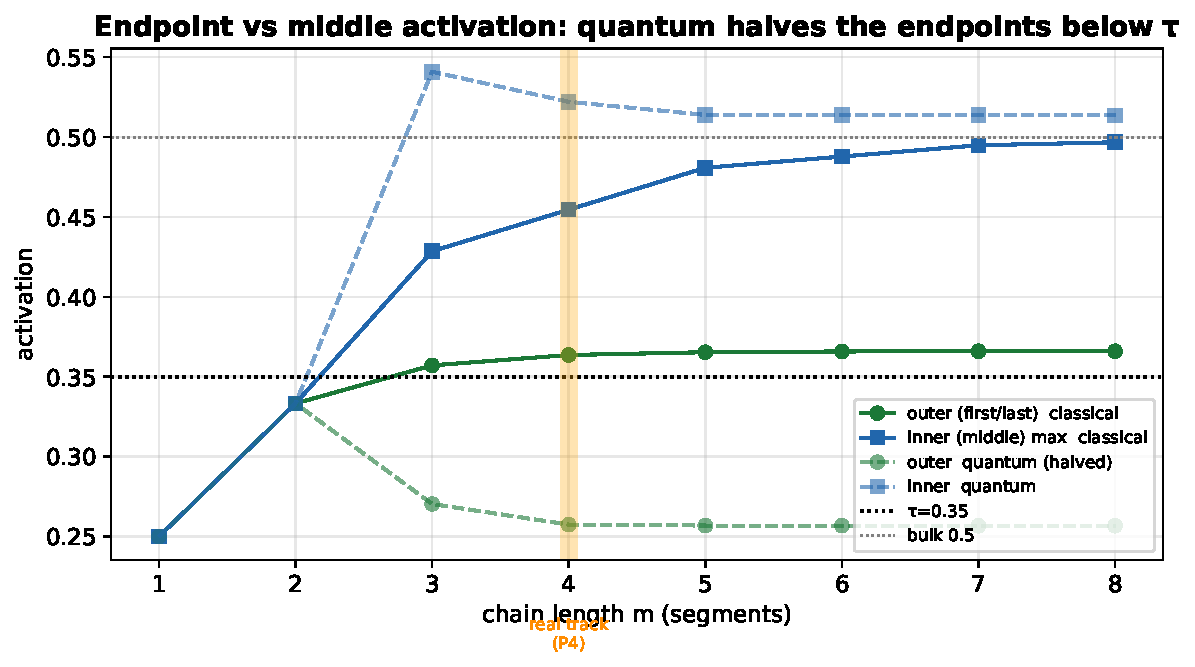
\includegraphics[width=0.75\textwidth]{chain_amplitude_ladder.pdf}
\caption{The chain ladder and the endpoint halving. Classical outer
activation climbs eq.~\eqref{eq:ladder} toward $0.366$ (above $\tau$);
the 1BQF response drops the $P_4$ outer level to $0.258$, below the
fixed threshold. This is the origin of the fixed-$\tau$ efficiency
plateau, and the reason 1BQF headlines use the efficiency-first
working point.}
\label{fig:ladder}
\end{figure}

The second consequence is that coupled false segments pass. A false
segment that accidentally couples to the graph moves off the
$\lambda=s$ line, out of the zero, and into the passband. The notch
has no second zero to spend on it. As density or acceptance width
grows, the coupled-false population grows, and the 1BQF's false rate
grows with it. The 1BQF is, precisely, the statement that unconnected
fakes are exactly removable; everything in this paper beyond
section~\ref{sec:qsvt} is about the connected ones.

On success probability: the kept-branch probability scales as
$P_{\rm anc}\approx 0.25/T$ on this problem, since the uniform input
spreads over $4T^2$ segments of which order $T$ carry surviving
amplitude, so shot budgets grow linearly in $T$ and amplitude
amplification buys the usual quadratic discount.\footnote{The $0.25$
constant is the analytic estimate for the uniform input; the comb's
analogous constant, $\approx0.44$, is directly measured
(section~\ref{sec:comb:resources}).} These costs carry over
essentially unchanged to the polynomial filters below, which is why I
defer resource accounting to section~\ref{sec:comb:resources}.

% ══════════════════════════════════════════════════════════════════════════════
\section{From one bit to any polynomial: the QSVT construction}
\label{sec:qsvt}

The promotion from eq.~\eqref{eq:notch} to an arbitrary polynomial
response rests on three standard ingredients: block encoding,
qubitization, and a linear combination of unitaries (LCU). I assemble
them here in the concrete, real-arithmetic form used by the
simulations. Readers who trust the QSVT
literature~\cite{gslw2019,lowchuang2019,childs2012,martyn2021} can
skim to the resource summary in section~\ref{sec:qsvt:resources}; the
details are included because the paper's cost claims (qubit counts,
walk calls, success probabilities) are read directly off this
construction.

\subsection{Block encoding and the qubitization walk}

Rescale the Hamiltonian affinely so its spectrum fits in $[-1,1]$:
$X=(A-c_0 I)/c_1$ with $c_0$ the spectrum centre and $c_1$ slightly
more than its half-width\footnote{The implementation pads the
user-supplied spectral bounds by a few percent; an early campaign bug
taught us that the polynomial's fit domain must exceed the padded
bounds or the constructor rightly refuses.}. A block encoding is a
unitary that hides $X$ in its top-left corner:
\begin{equation}
U=\begin{pmatrix} X & \sqrt{I-X^{2}}\\[2pt] \sqrt{I-X^{2}} & -X
\end{pmatrix},
\label{eq:dilation}
\end{equation}
acting on the segment register plus one \emph{dilation} qubit. The
picture I find most useful is a rotation in each eigenplane: for every
eigenvalue $x$ of $X$ there is a two-dimensional invariant subspace in
which $U$ rotates by the angle $\arccos x$.

The word \emph{walk} deserves an explanation, because nothing in this
paper has moved yet and the term is imported jargon. A walk operator
is simply a fixed unitary that one applies over and over, taking one
``step'' per application, in analogy with a classical random walk
where one transition matrix is applied repeatedly. The useful property
is what repetition does. Because $U$ rotates each eigenplane by
$\arccos x$, applying the walk $k$ times rotates it by $k\arccos x$,
and the component that ends where it started is
$\cos(k\arccos x)$ --- which is precisely the $k$-th Chebyshev
polynomial $T_k(x)$. One application of the walk knows only $x$;
$k$ applications know $T_k(x)$. Repetition of a single fixed circuit
therefore \emph{generates a polynomial family}, one degree per step,
and that is the entire mechanism by which a quantum computer applies
polynomials of a matrix without ever diagonalising it. Formally, the
\emph{qubitization walk} $W=(Z\otimes I)\,U$ (the extra sign
$Z$ on the dilation qubit turns the reflections of $U$ into clean
rotations) has the defining property
\begin{equation}
\big\langle 0\big|\,W^{k}\,\big|0\big\rangle_{\rm dil}=T_{k}(X),
\label{eq:walkcheb}
\end{equation}
where $T_k$ is the $k$-th Chebyshev polynomial and the bra-ket
projects the dilation qubit onto $|0\rangle$.
Equation~\eqref{eq:walkcheb} is exact, with no Trotterization and no
error terms, and every operator in it is real, so the entire
simulation can run in real arithmetic on orthogonal matrices. Walking
$k$ steps and looking at the undeflected component applies the $k$-th
Chebyshev polynomial of the Hamiltonian; that is the whole theorem.

\subsection{Summing the series: LCU}

A degree-$d$ response $p(X)=\sum_{k=0}^{d}c_k T_k(X)$ is then a
weighted sum of walk powers. Introduce an index register of
$m=\lceil\log_2(d{+}1)\rceil$ qubits, prepare
$|{\rm prep}\rangle\propto\sum_k\sqrt{|c_k|}\,|k\rangle$, apply
$W^{k}$ controlled on the index (in practice: controlled powers
$W^{2^j}$), undo the preparation, and post-select the index and
dilation registers on zero. The surviving register state is
$\propto p(X)|u\rangle$ with success probability
\begin{equation}
P_{\rm anc}=\frac{\big\lVert p(X)\,|u\rangle\big\rVert^{2}}
{\big(\sum_k |c_k|\big)^{2}} ,
\label{eq:psucc}
\end{equation}
the usual LCU price: the one-norm of the coefficient vector. The 1BQF
is recovered, exactly, as the $d=1$ row of this table ($\cos$ is
$T_1$ of the appropriately rescaled operator), which is the formal
content of the claim that this paper continues rather than replaces
its predecessors.

Simulation-side, eq.~\eqref{eq:walkcheb} gives a matrix-free
evaluator: $p(A)\mathbf{b}$ by the Chebyshev three-term recursion on
sparse matrix-vector products, $\mathcal{O}(d\cdot{\rm nnz}(A))$
flops. In a persisted benchmark of the production configuration the
$d=40$ comb solve runs in $1.2$--$1.7$\,s at $T=1000$
($n=4\times10^{6}$), and the evaluator agrees with the full qiskit
circuit and with a gate-streaming evaluation to better than
$10^{-14}$ at circuit-affordable size (three-way maximum
discrepancy $8\times10^{-15}$). All large-$T$ results below use this
exact evaluator; nothing in this paper relies on an approximate
simulation of the quantum readout.

\subsection{Resource summary}
\label{sec:qsvt:resources}

For a degree-$d$ filter on an event of $T$ tracks:
\begin{itemize}[leftmargin=2em]
\item \textbf{Width}: $n_{\rm sys}=\lceil\log_2 4T^2\rceil$ system
qubits $+\,1$ dilation $+\,m=\lceil\log_2(d{+}1)\rceil$ index qubits.
With the production degree $d=40$ this is 21 qubits at $T=50$ rising
to 29 at $T=1000$. Width is cheap, and grows only logarithmically.
\item \textbf{Depth}: $d$ controlled walk calls per coherent
repetition, times $\mathcal{O}(1/\sqrt{P_{\rm anc}})$
amplitude-amplification rounds.
\item \textbf{Success}: $P_{\rm anc}\propto 1/T$ (measured constant
$\approx0.44$ for the comb of section~\ref{sec:comb}), so total walk
calls scale as $d\sqrt{T}$.
\end{itemize}
The quantum content of this paper is this resource profile; the
response functions themselves are classically simulable by the same
recursion, and I return to what that does and does not concede in
section~\ref{sec:limits:dequant}.

% ══════════════════════════════════════════════════════════════════════════════
\section{Fitting the polynomial to the clean events: the line comb}
\label{sec:comb}

\subsection{The design insight: the true spectrum is discrete}

Here is the observation that turns QSVT from a mathematical
possibility into a design tool. On this detector geometry every true
track has exactly five hits, hence exactly four segments, hence, by
eq.~\eqref{eq:p4lines}, exactly the same four eigenvalues. The true
spectrum of the entire event, however many thousand tracks it
contains, is four discrete lines. We are not trying to pass a region
of the spectrum; we are trying to pass four known radio stations, and
everything between them is static.

My first design did not understand this. A band-limited approximate
inverse ($\approx1/\lambda$ across a contiguous band containing the
true lines, zero outside) works beautifully at low multiplicity and
then fails exactly where it matters: as $T$ grows, accidental tangles
of false segments produce eigenvalues throughout the band, and a band
design passes them all. At fixed threshold its false rate reached tens
of percent by $T=400$, worse than classical.\footnote{A useful
failure: it taught us that the exploitable structure is the
discreteness of the geometry-pinned true spectrum, not its location.}
The production design is therefore a \emph{line comb}: narrow Gaussian
passes of half-width $h_w$, weighted $\propto1/\lambda$, centred at
the four lines $s-2\cos(k\pi/5)$ only, fitted as a bounded Chebyshev
series of degree $d$. The defaults, fixed once by a two-dimensional
$(d,h_w)$ scan and never tuned per event, are $d=40$, $h_w=0.18$.

Why does a width of $0.18$ work? The nearest systematically-populated
false lines, the $P_3$ bridge modes at $\{s-\sqrt2,\,s,\,s+\sqrt2\}$,
sit $\gtrsim0.2$ away from the true lines, so the comb threads the
gap; and the resolution law of a degree-$d$ Chebyshev series, features
no narrower than $\approx 2W/d$ on a domain of half-width $W$, makes
$d=40$ sufficient for $h_w=0.18$ on the clean-event domain. Degree,
width, and line spacing are one budget, and this is the budget the
noisy events of section~\ref{sec:fit} will re-open.

\subsection{Clean-event results}
\label{sec:comb:results}

On the fixed-acceptance ($\varepsilon=2$\,mrad), $\gamma=3$ study, the
canonical benchmark of the programme, with events and solutions shared
segment-for-segment across all three solvers through a common data
pipeline, the picture at the fixed threshold $\tau=0.35$ is:
\begin{itemize}[leftmargin=2em]
\item \textbf{Classical}: efficiency $100\%$ throughout (the minimum
true amplitude $4/11$ clears $\tau$ at every $T$); false rate grows
from $\approx0$ at low $T$ to $2.25\%$ at $T=400$ and $20.5\%$ at
$T=1000$ as the $\mathcal{O}(T^2)$ false pairing feeds the active
set.
\item \textbf{1BQF}: the fixed-$\tau$ efficiency plateau of
section~\ref{sec:onebit} ($74.7\%$ at $T=400$, the endpoint cut);
false rate at or just below classical ($1.73\%$ at $T=400$, $18.8\%$
at $T=1000$).
\item \textbf{Comb}: efficiency $97$--$100\%$ with false rate
$\le0.02\%$ through $T=400$ (zero to a few false actives per event
where the classical solver admits tens), rising to $0.17\%$ at
$T=700$ and $0.9\%$ at $T=1000$ against the classical $20.5\%$, at
efficiency $92.1\%$.
\end{itemize}

\begin{figure}[t]
\centering
\captionsetup{width=0.92\textwidth}
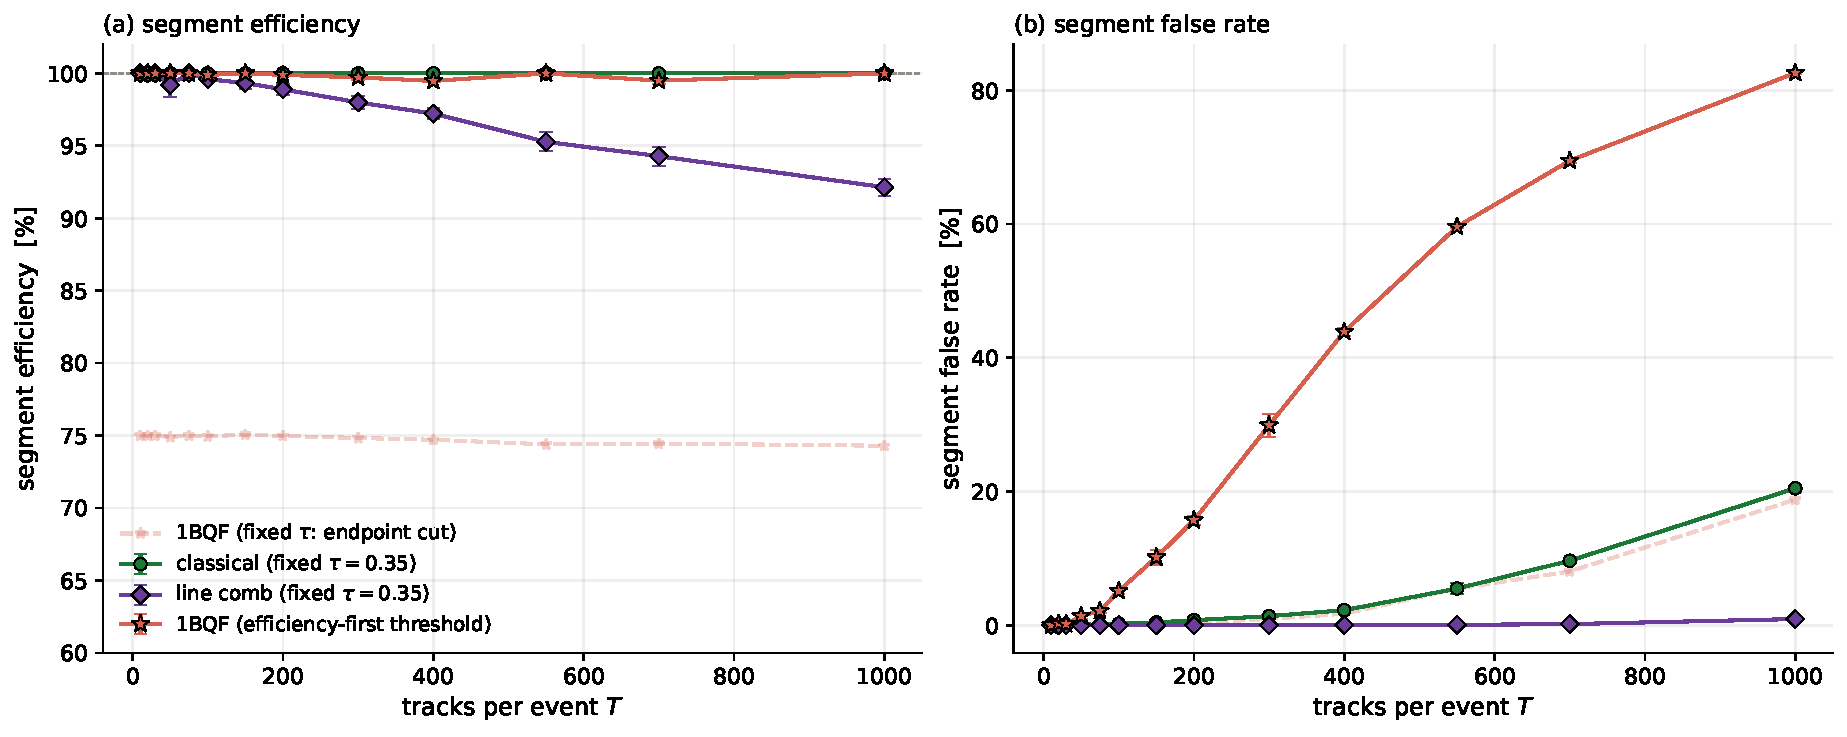
\includegraphics[width=0.95\textwidth]{clean_headline.pdf}
\caption{The clean-toy headline ($\gamma=3$, fixed
$\varepsilon=2$\,mrad, no hit drop): (a) segment efficiency and (b)
segment false rate against multiplicity, for the classical solver and
the line comb at the fixed threshold and the 1BQF at its
efficiency-first working point (its fixed-$\tau$ curve is kept faded:
the $\approx75\%$ plateau is the endpoint cut of
section~\ref{sec:onebit}, not lost physics). Error bars are standard
errors over event repetitions.}
\label{fig:clean2x2}
\end{figure}

At the efficiency-first working point the comb wins clearly through
$T=400$ ($1.3\%$ vs classical $3.1\%$ on matched fresh solves), but
at extreme density the composition effect dominates everyone: the
false-to-true ratio $n_F/n_T\approx T-1$ converts even excellent
per-segment separation into a growing impurity, and by $T=1000$ the
efficiency-first false rates cross ($\approx21\%$ comb vs $17.5\%$
classical, crossover near $T=700$).\footnote{The crossover is robust;
its size is aggregation-dependent. A whole-store aggregate reads the
classical efficiency-first false rate at $T=1000$ as low as $10\%$.
Both sources agree the comb no longer wins at the efficiency-first
point beyond $T\approx700$, which is the operative statement.} The
two regimes, fixed-$\tau$ where the comb wins by an order of
magnitude and more, and the strict efficiency-first point at extreme
density where composition flattens everyone, bracket the operational
truth.

The comb's amplitude picture explains the numbers. Under the comb
response the false population collapses to $\lesssim10^{-2}$ of the
true median (the passes reject everything off the lines), while the
true band stays tight around its classical profile: the $1/\lambda$
weighting inside the passes preserves the chain shape rather than
reshaping it as the single cosine does. Where the 1BQF splits the
true population and the classical solver drags a false tail across
the threshold, the comb simply leaves a gap.

\subsection{Hit inefficiency: the first appearance of fragments}
\label{sec:comb:drop}

Dropping $1\%$ of hits breaks $\approx5\%$ of tracks into fragments:
chains of one, two, or three segments whose spectra
(section~\ref{sec:toy:spectrum}) are \emph{not} on the four $P_4$
lines. The comb, by design, does not pass them. Per-class efficiency
under the production comb is $100\%$ on intact tracks and $0\%$ on
every fragment class, which is why its overall efficiency reads
$94.0\%$ rather than $97$--$98\%$ at $T=400$ under drop. Extending
the comb with passes at the fragment lines does not help: it
re-admits their false spectral twins wholesale (a $P_2$ fragment and
a false pair are the same matrix, figure~\ref{fig:twins}), so
fragments are a spectral
floor \emph{on this Hamiltonian}, the first appearance of the twin
obstruction that
section~\ref{sec:fit} meets at full strength --- and that
section~\ref{sec:fit:occ} shows an operator modification can
lift. Recovery on the unmodified Hamiltonian must come from
information a spectral filter
cannot see, namely hit-level constraint information, and that is
classical post-processing, outside the scope of this
paper.\footnote{An earlier version of this study paired a
hit-occupancy recovery gate with the comb alone; it was retired as
mission creep (no other solver received the same help, and the tool
is orthogonal to the spectral question). Classical post-selection is
developed and reported separately in the programme's occupancy
study.}

\subsection{Resource scaling and the depth ladder}
\label{sec:comb:resources}

Measured on the shared events: total width 21 qubits at $T=50$ to 29
at $T=1000$; success probability $P_{\rm anc}\approx0.44/T$; walk
calls per amplified repetition
$d\cdot\pi/(4\sqrt{P_{\rm anc}})\propto d\sqrt T$. Two findings
sharpen the budget. A half-resolved comb at $d=16$ matches the
$d=40$ metrics up to $T=700$ at an approximately $T$-independent
$P_{\rm anc}\approx6\%$, about fifty total walk calls, flat in $T$,
because partially-merged passes still cover the four lines while
rejecting the bulk. And the degree axis is not monotonic:
intermediate degrees ($d\approx20$--$32$) can cliff at the
efficiency-first working point through Chebyshev fit pathologies, so
every production degree must be validated, not interpolated.

\begin{figure}[t]
\centering
\captionsetup{width=0.80\textwidth}
\begin{subfigure}[t]{0.80\textwidth}
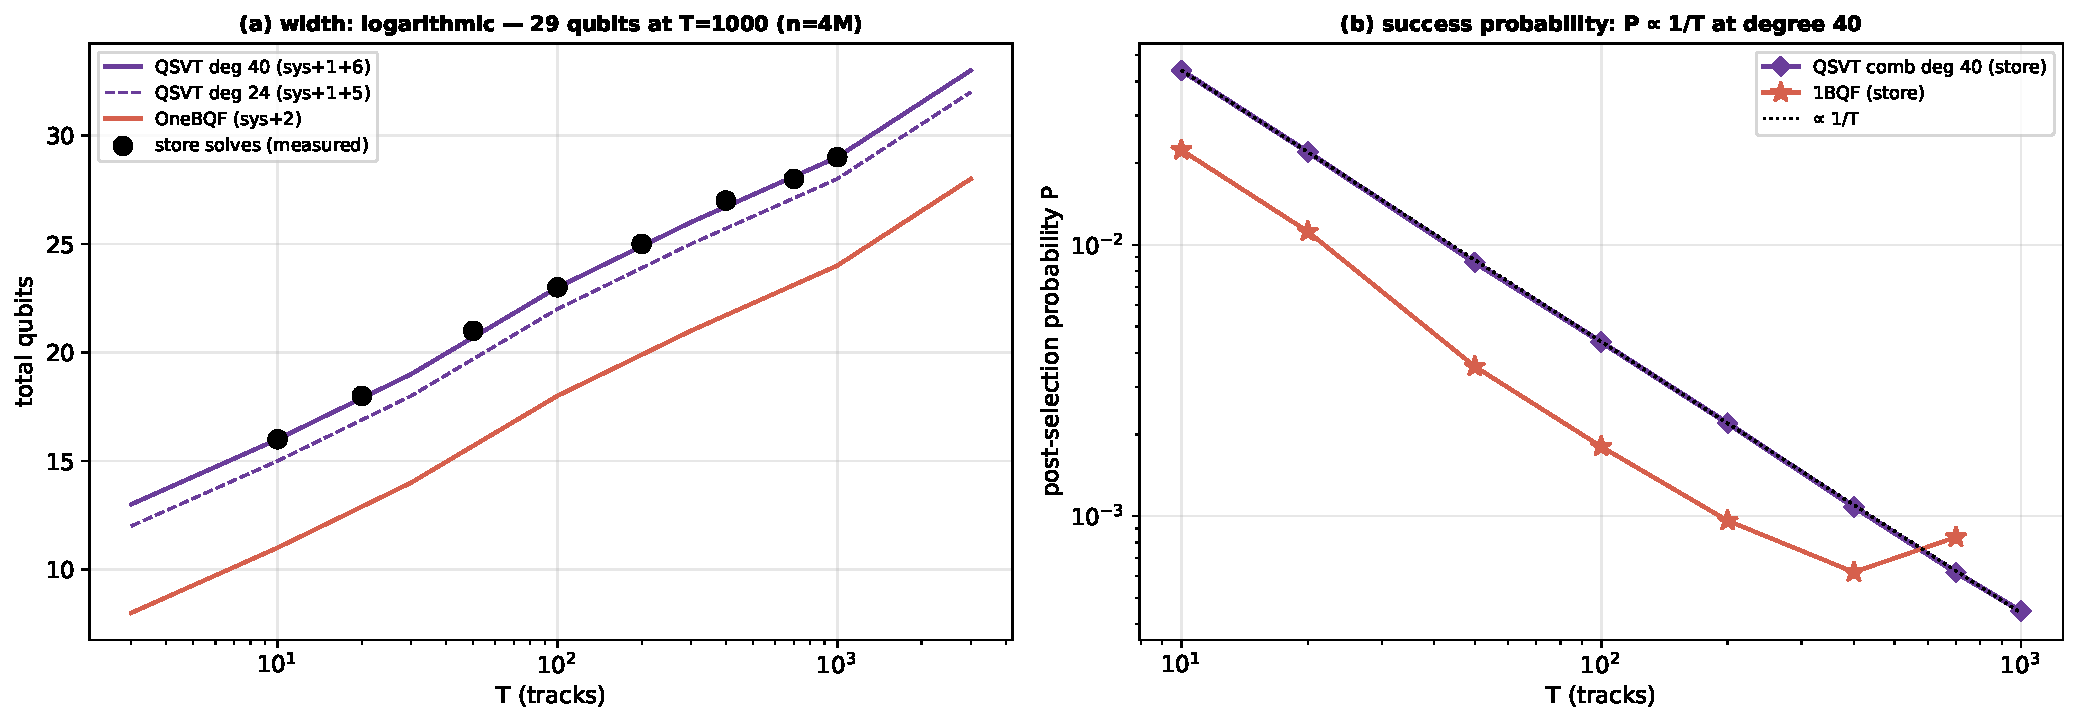
\includegraphics[width=\textwidth]{qsvt_width_and_P.pdf}
\caption{Register width and success probability.}
\end{subfigure}\\[6pt]
\begin{subfigure}[t]{0.80\textwidth}
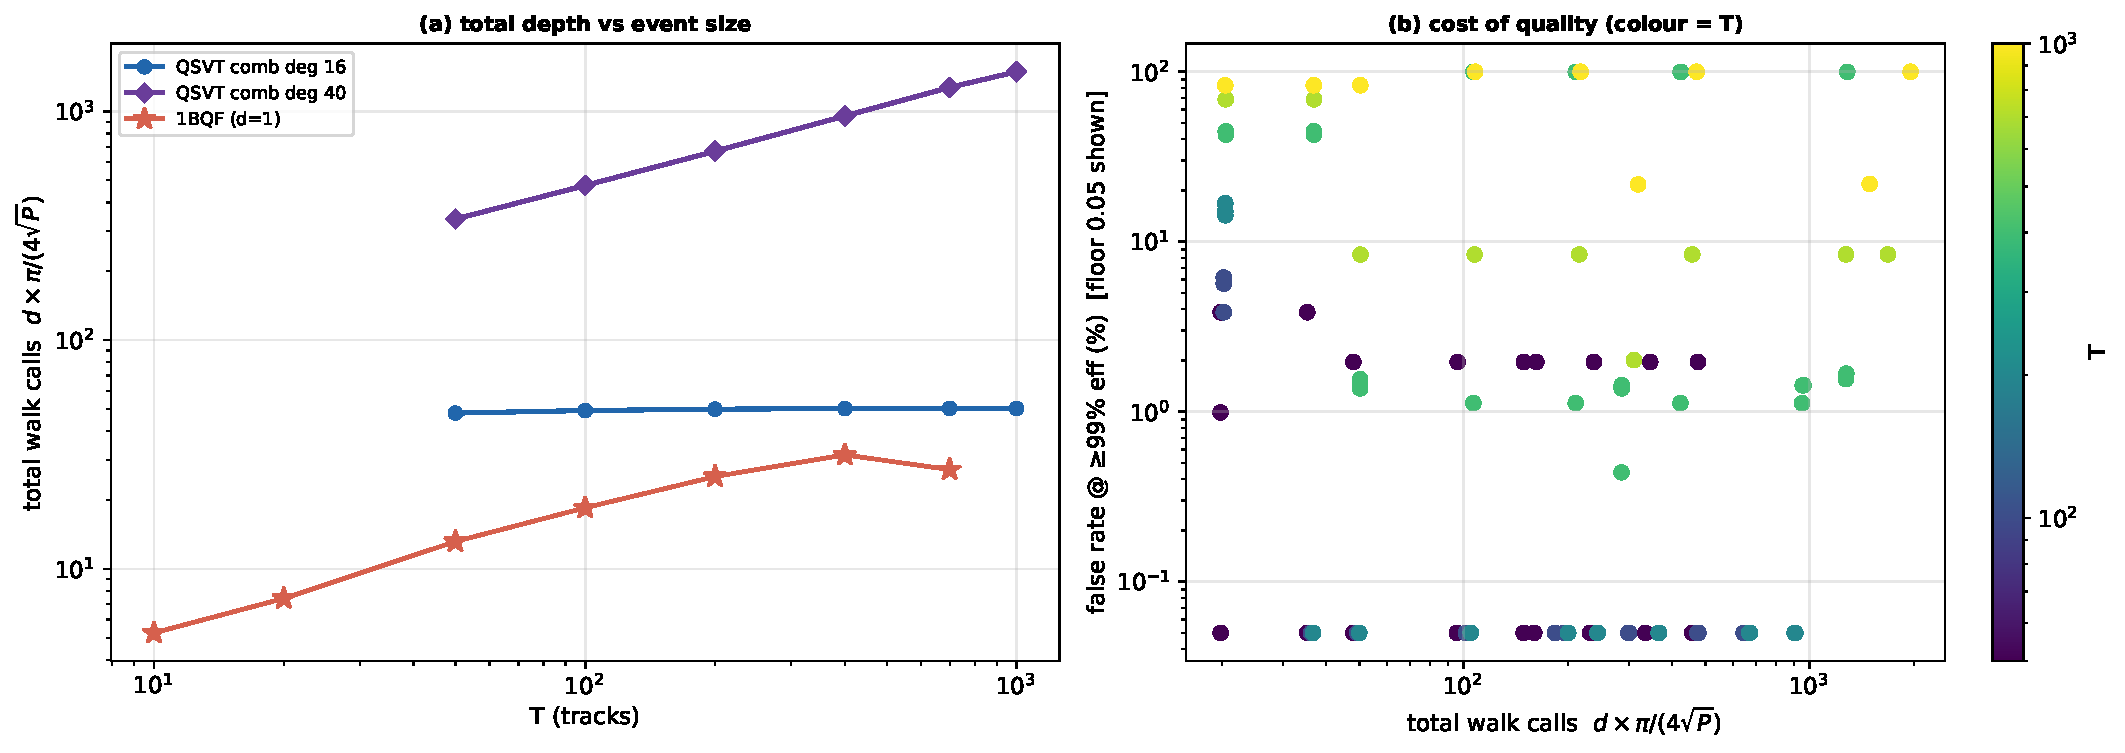
\includegraphics[width=\textwidth]{qsvt_total_depth.pdf}
\caption{Total walk calls (depth).}
\end{subfigure}
\caption{Measured resource scaling of the comb on the shared events:
width grows logarithmically (21 qubits at $T=50$ to 29 at $T=1000$);
success probability falls as $\approx0.44/T$; amplified walk calls
grow as $d\sqrt T$, with the half-resolved $d=16$ comb holding a
$T$-independent $\approx50$-call budget to $T=700$.}
\label{fig:resources}
\end{figure}

\subsection{Spectral twins and the floor theorem}
\label{sec:comb:limits}

The most important structural limit on the whole filter family
deserves its own name and its own picture. Call two segment clusters
\emph{spectral twins} when their compatibility graphs are isomorphic:
the same number of segments, connected in the same pattern, regardless
of where the segments physically are or whether they belong to a real
track. Because $A$ acts block-diagonally over connected components,
each cluster contributes a sub-block of $A$, and twin clusters
contribute \emph{the same sub-block up to relabelling} (permutation
similarity). The consequence is the \emph{floor theorem}: for every
function $f$, $f(A)\mathbf{b}$ assigns twin clusters identical
amplitudes, because permutation similarity commutes with matrix
functions and $\mathbf{b}$ is uniform on every cluster. No response,
fitted or otherwise, and no classical amplitude scoring, can tell
twins apart: whatever passes one passes the other.

Figure~\ref{fig:twins} draws the pair of twins that will matter most
in this paper. A true two-segment fragment (three surviving hits of a
broken track) and a false pair (two fake segments that happen to
continue one another inside the acceptance) are physically completely
different objects; but both are two segments sharing one hit, both
produce the same $2\times2$ sub-block of $A$, and both therefore sit
on exactly the eigenvalue lines $s\mp1$ with exactly the same
amplitudes. On clean events twins are rare (an exhaustive scan of the
$T\le200$ events finds none; $0.6\%$ of true segments by $T=400$ with
the acceptance widened to $4$\,mrad), but they are the true ceiling of
the design, and under noise they return, as a population, in
section~\ref{sec:fit}.

\begin{figure}[t]
\centering
\captionsetup{width=0.92\textwidth}
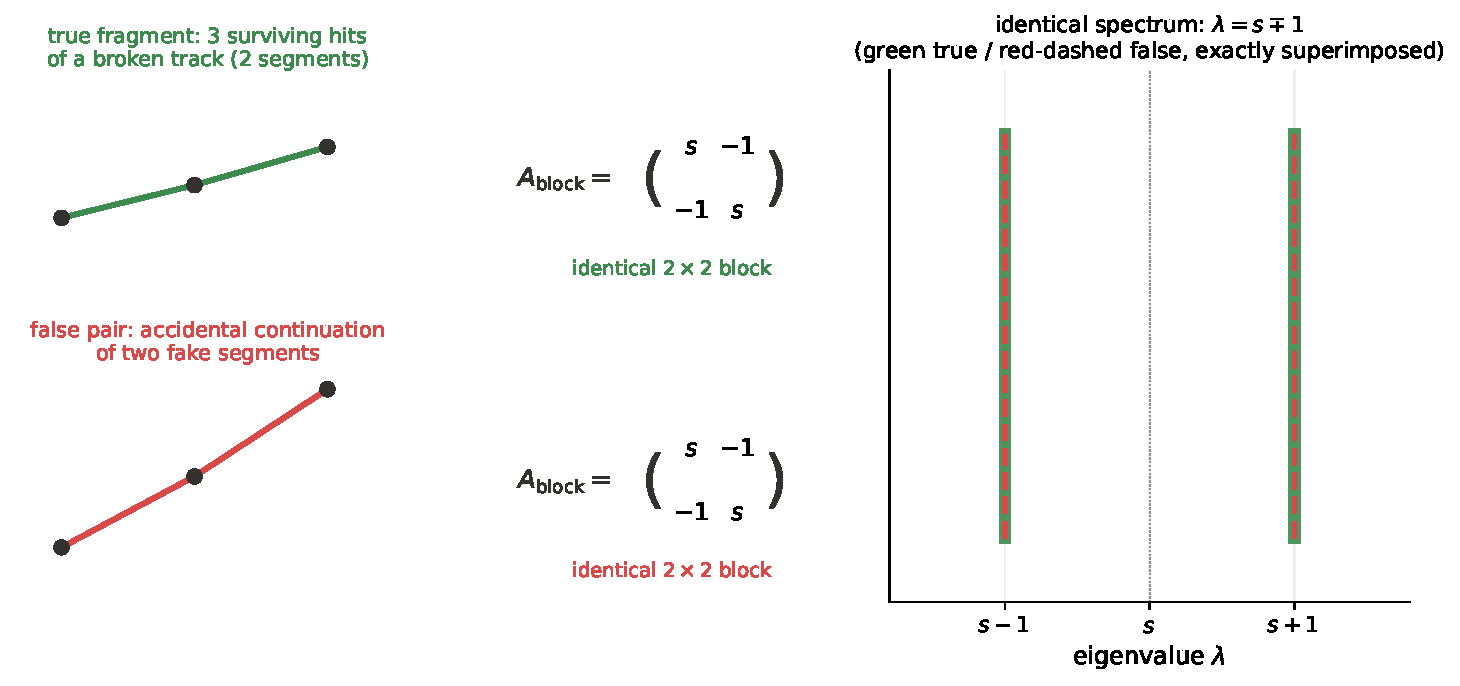
\includegraphics[width=0.95\textwidth]{spectral_twins.pdf}
\caption{Spectral twins. A true fragment of a broken track (top) and
an accidental false pair (bottom) have isomorphic compatibility
graphs, hence identical $2\times2$ sub-blocks of $A$, hence exactly
the same eigenvalues and amplitudes. Every function of $A$ treats
them identically; this is the floor theorem, and under noise it
becomes the fragment floor of section~\ref{sec:fit}.}
\label{fig:twins}
\end{figure}

Two further structural results complete the clean-toy picture. The
\emph{shared-line theorem}: the odd modes of a contaminated
five-segment chain coincide exactly with the $s\pm\sqrt3$ lines of
the three-pronged hub $K_{1,3}$, so no comb can null both populations
independently; pass menus trade one against the other with a fixed
exchange rate. And the \emph{mirror tax}: a chain-reflection symmetry
forces the false extension of a recovered cluster to the
recovered-true amplitude level, so recovery passes always buy their
efficiency at a false-rate premium. Together these results closed the
clean-toy design question. The production comb is optimal up to
provable exceptions, and further progress must come from changing
the operator or leaving the spectral domain, which is exactly where
the rest of this paper goes.

% ══════════════════════════════════════════════════════════════════════════════
\section{The heavy-noise operating point}
\label{sec:noise}

From here on the operating point is the heavy configuration:
$\sigma_{\rm scatt}=10^{-4}$, $\sigma_{\rm res}=20\,\mu$m, hit drop
$1\%$, at $T=200$, with the acceptance set by the kink formula to
$\varepsilon=6.3$\,mrad. Three reps of every event are used
throughout; where a single event is dissected, it is rep~0.

The acceptance width is the story. At $\varepsilon=2$\,mrad a false
segment rarely finds an angular partner; at $6.3$\,mrad the
compatibility graph fills with small false structures. Two facts
about that graph, both established by direct decomposition of the
solved events, control everything downstream:
\begin{enumerate}[leftmargin=2em]
\item \textbf{There is no giant tangle.} The compatibility graph at
heavy $T=200$ splits into $869$ nontrivial connected
components of at most $17$ segments, floating in a sea of
$155{,}371$ isolated segments (rep~0). Noise, at this operating
point, buys many small motifs rather than one big mess, and small
components mean the entire spectrum is computable exactly, component
by component, with dense eigensolvers. Every spectral statement in
sections~\ref{sec:occupancy}--\ref{sec:fit} is exact, not
approximate. Figure~\ref{fig:tangles} shows what these components
actually look like in the detector: the component-size distribution,
and real examples drawn from the event, from a pure-false pair to
the largest seventeen-segment tangle. Seen at the micron scale of
their internal kinks, the ``tangles'' are bundles of near-collinear
competitors --- exactly the structures the widened acceptance
admits.
\item \textbf{The false actives are motif-borne.} At the classical
efficiency-first working point the event has $2238$ active segments
of which $1454$ are
false; those false actives live in $707$ components that contain,
between them, only $142$ true segments. Ninety percent of the
false-active population sits in essentially pure-false motifs
(pairs, triples, short bridges), not entangled with true tracks at
all. Spectrally, this population lands exactly where the motif
dictionary of figure~\ref{fig:motifs} says it must:
figure~\ref{fig:pileup} shows the measured per-mode solution weight
of the event against $\lambda$, with the false weight piled up on
the pair line $s-1$ and the triple lines $s\pm\sqrt2$, interleaving
but not touching the four true lines.
\end{enumerate}

\begin{figure}[t]
\centering
\captionsetup{width=0.95\textwidth}
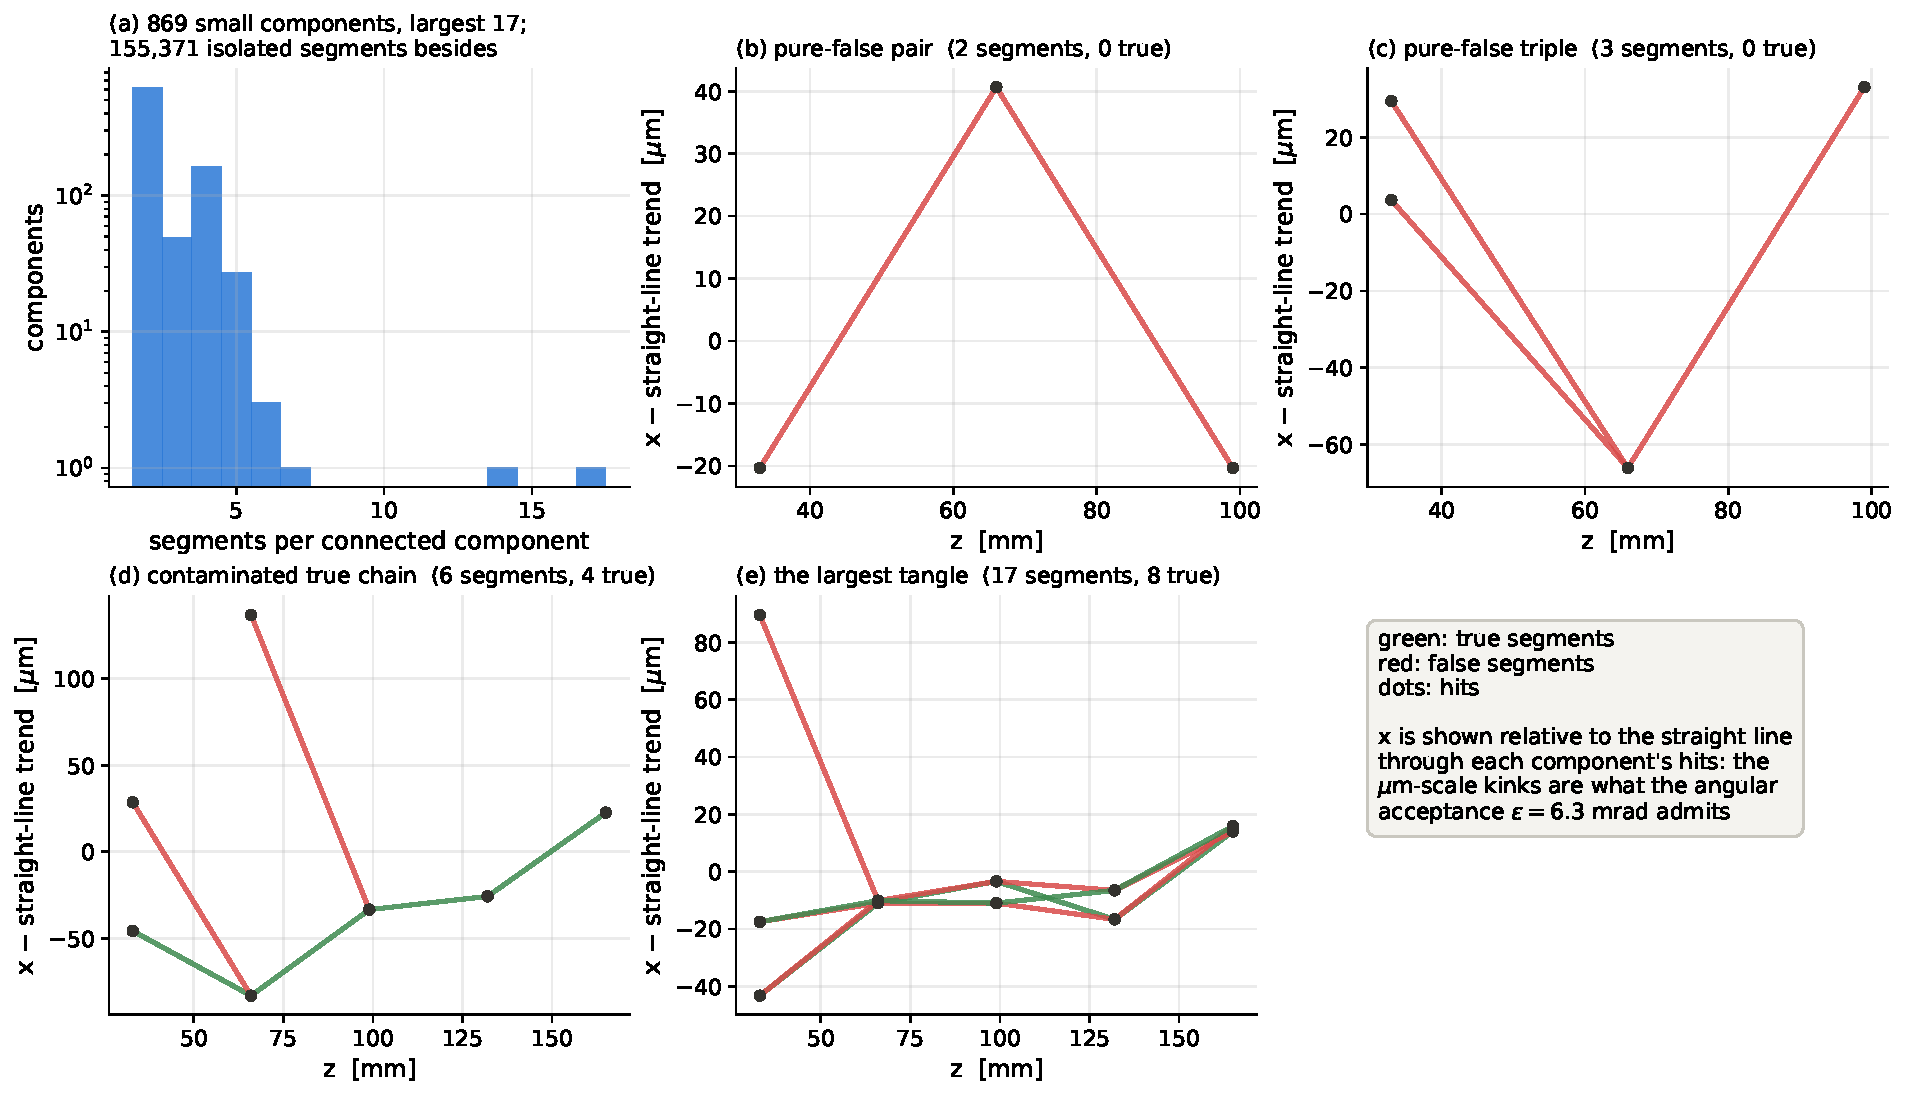
\includegraphics[width=0.98\textwidth]{tangle_gallery.pdf}
\caption{The heavy-noise compatibility graph, seen directly (heavy
$T=200$, rep~0). (a) Component-size distribution: many small motifs,
no giant component. (b--e) Real components drawn in the detector,
with the straight-line trend subtracted so the micron-scale kinks are
visible: a pure-false pair, a pure-false triple, a true chain with
false contamination, and the largest tangle in the event (17
segments, 8 true). Green segments are true, red false.}
\label{fig:tangles}
\end{figure}

\begin{figure}[t]
\centering
\captionsetup{width=0.90\textwidth}
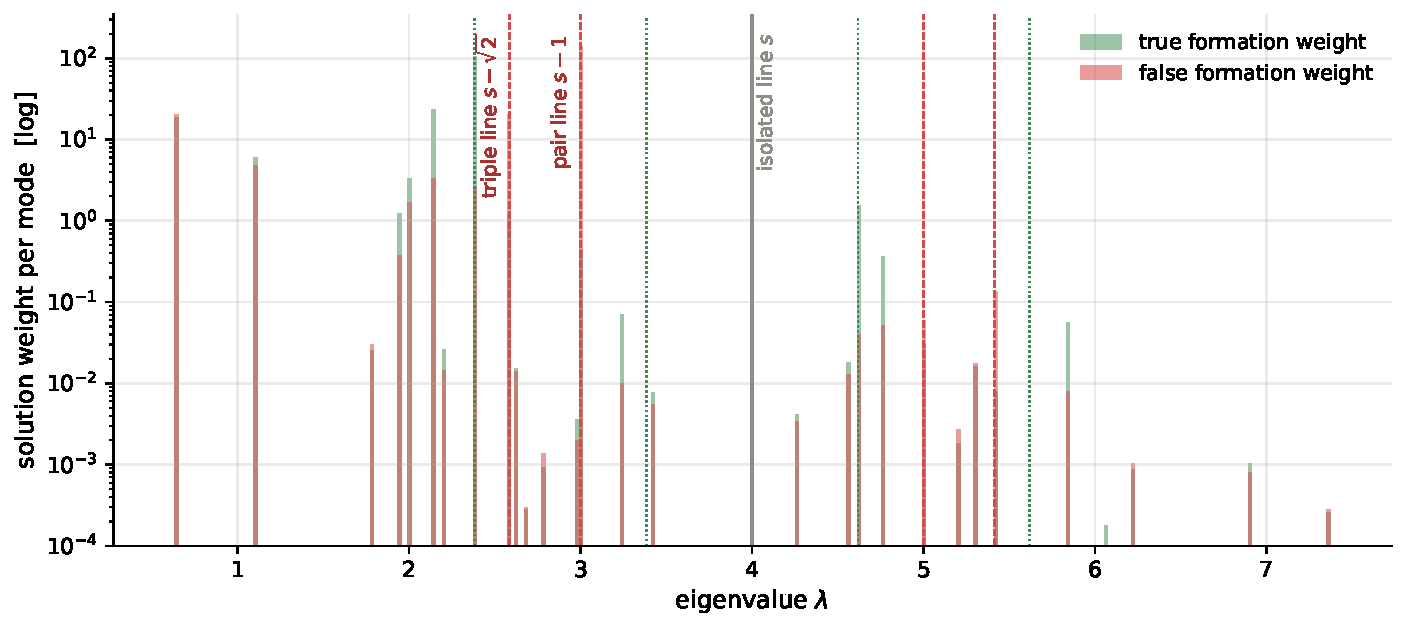
\includegraphics[width=0.92\textwidth]{measured_pileup.pdf}
\caption{The measured spectral pile-up of the heavy $T=200$ event
(rep~0), computed exactly by per-component diagonalisation: solution
weight per mode against $\lambda$, split into true (green) and false
(red) content. The false weight concentrates on the pair line $s-1$
and the triple lines $s\pm\sqrt2$ of the motif dictionary
(figure~\ref{fig:motifs}), close to but never on the four true-track
lines (green dotted).}
\label{fig:pileup}
\end{figure}

The solver scoreboard at this point makes uncomfortable reading. At
the efficiency-first working point the classical false rate is
$0.65$; the 1BQF's is $0.65$ as
well, since the notch's one zero still annihilates the isolated bulk
while every false \emph{active} is by definition coupled, off the
line, and untouched. The clean-event comb, designed for a $2$\,mrad
world where false structures barely exist, fails too: the
wide acceptance populates false motif lines (figure~\ref{fig:pileup})
inside its pass windows. The important statement here is the
diagnosis: at heavy noise all three solvers fail for the same
reason, a false population that has moved onto spectral lines the
designs were never told about --- and the cure, developed in
section~\ref{sec:fit}, is to measure those lines and refit the
response to them. The classical literature also offers two
Hamiltonian terms as candidate cures, occupancy and bifurcation. The
next two sections take them in turn; neither behaves the way its
classical reputation suggests, and neither can be judged separately
from the refit.

% ══════════════════════════════════════════════════════════════════════════════
\section{The occupancy term}
\label{sec:occupancy}

\subsection{The term}

Denby's original network~\cite{denby1988} constrains each hit to be
used by at most one selected segment per role. The quadratic form of
that constraint, per-hit occupancy, adds
$E_{\rm occ}=\alpha\sum_h(o_h-1)^2$ with $o_h=\sum_{s\ni h}x_s$,
which at the matrix level reads
\begin{equation}
A_{\rm occ}=A+4\alpha I+2\alpha B_{\rm all},\qquad
\mathbf{b}\to\mathbf{b}+4\alpha\mathbf{1},
\label{eq:occ}
\end{equation}
where $B_{\rm all}$ couples every pair of segments sharing a hit in
the same role: two segments departing the same hit, or two arriving
at it. Consecutive segments of one track share their interior hit in
opposite roles and are not coupled. The isolated attractor moves to
$(\delta+4\alpha)/(\gamma+\delta+4\alpha)$ and the threshold tracks
it.

\subsection{Classically it works; the notch it destroys}

On the heavy $T=200$ benchmark event the in-matrix occupancy term at
$\alpha=0.3$ does exactly what Denby promised: the classical
efficiency-first false rate falls from $0.650$ to $0.210$ at
efficiency $0.991$. If this paper were classical, the section would
end here with a recommendation.

For the 1BQF it is a disaster, and the mechanism is worth spelling
out because it generalises. The notch's power is that isolated false
segments sit exactly on its zero. The occupancy coupling
$2\alpha B_{\rm all}$ connects precisely those segments to their
co-hit neighbours, which is its job, and thereby moves them off the
zero. On the benchmark event the co-hit false bulk, notched to
amplitudes $\sim10^{-19}$ under the base Hamiltonian ($99\%$ of it
below $10^{-17}$), re-emerges under $A_{\rm occ}$ at amplitudes on
the true band: its 99th percentile rises to $1.5\times10^{-3}$
against a true median of $1.2\times10^{-3}$. The rank separation
collapses (1BQF AUC $0.996\to0.634$) and no threshold rescues it;
the full sweep shows every occupancy-1BQF operating point dominated
by the base-1BQF curve. Nor does the self-coupling $\gamma$ offer an
escape: the notch tracks the diagonal, distance-to-notch is
$\gamma$-invariant, and at the window-restoring $\gamma=236$ the
occupancy system is strictly worse. Post-selection tells the same
story: the occupancy term diverts the ancilla-conditioned
probability mass almost entirely onto false segments.

\begin{figure}[t]
\centering
\captionsetup{width=0.90\textwidth}
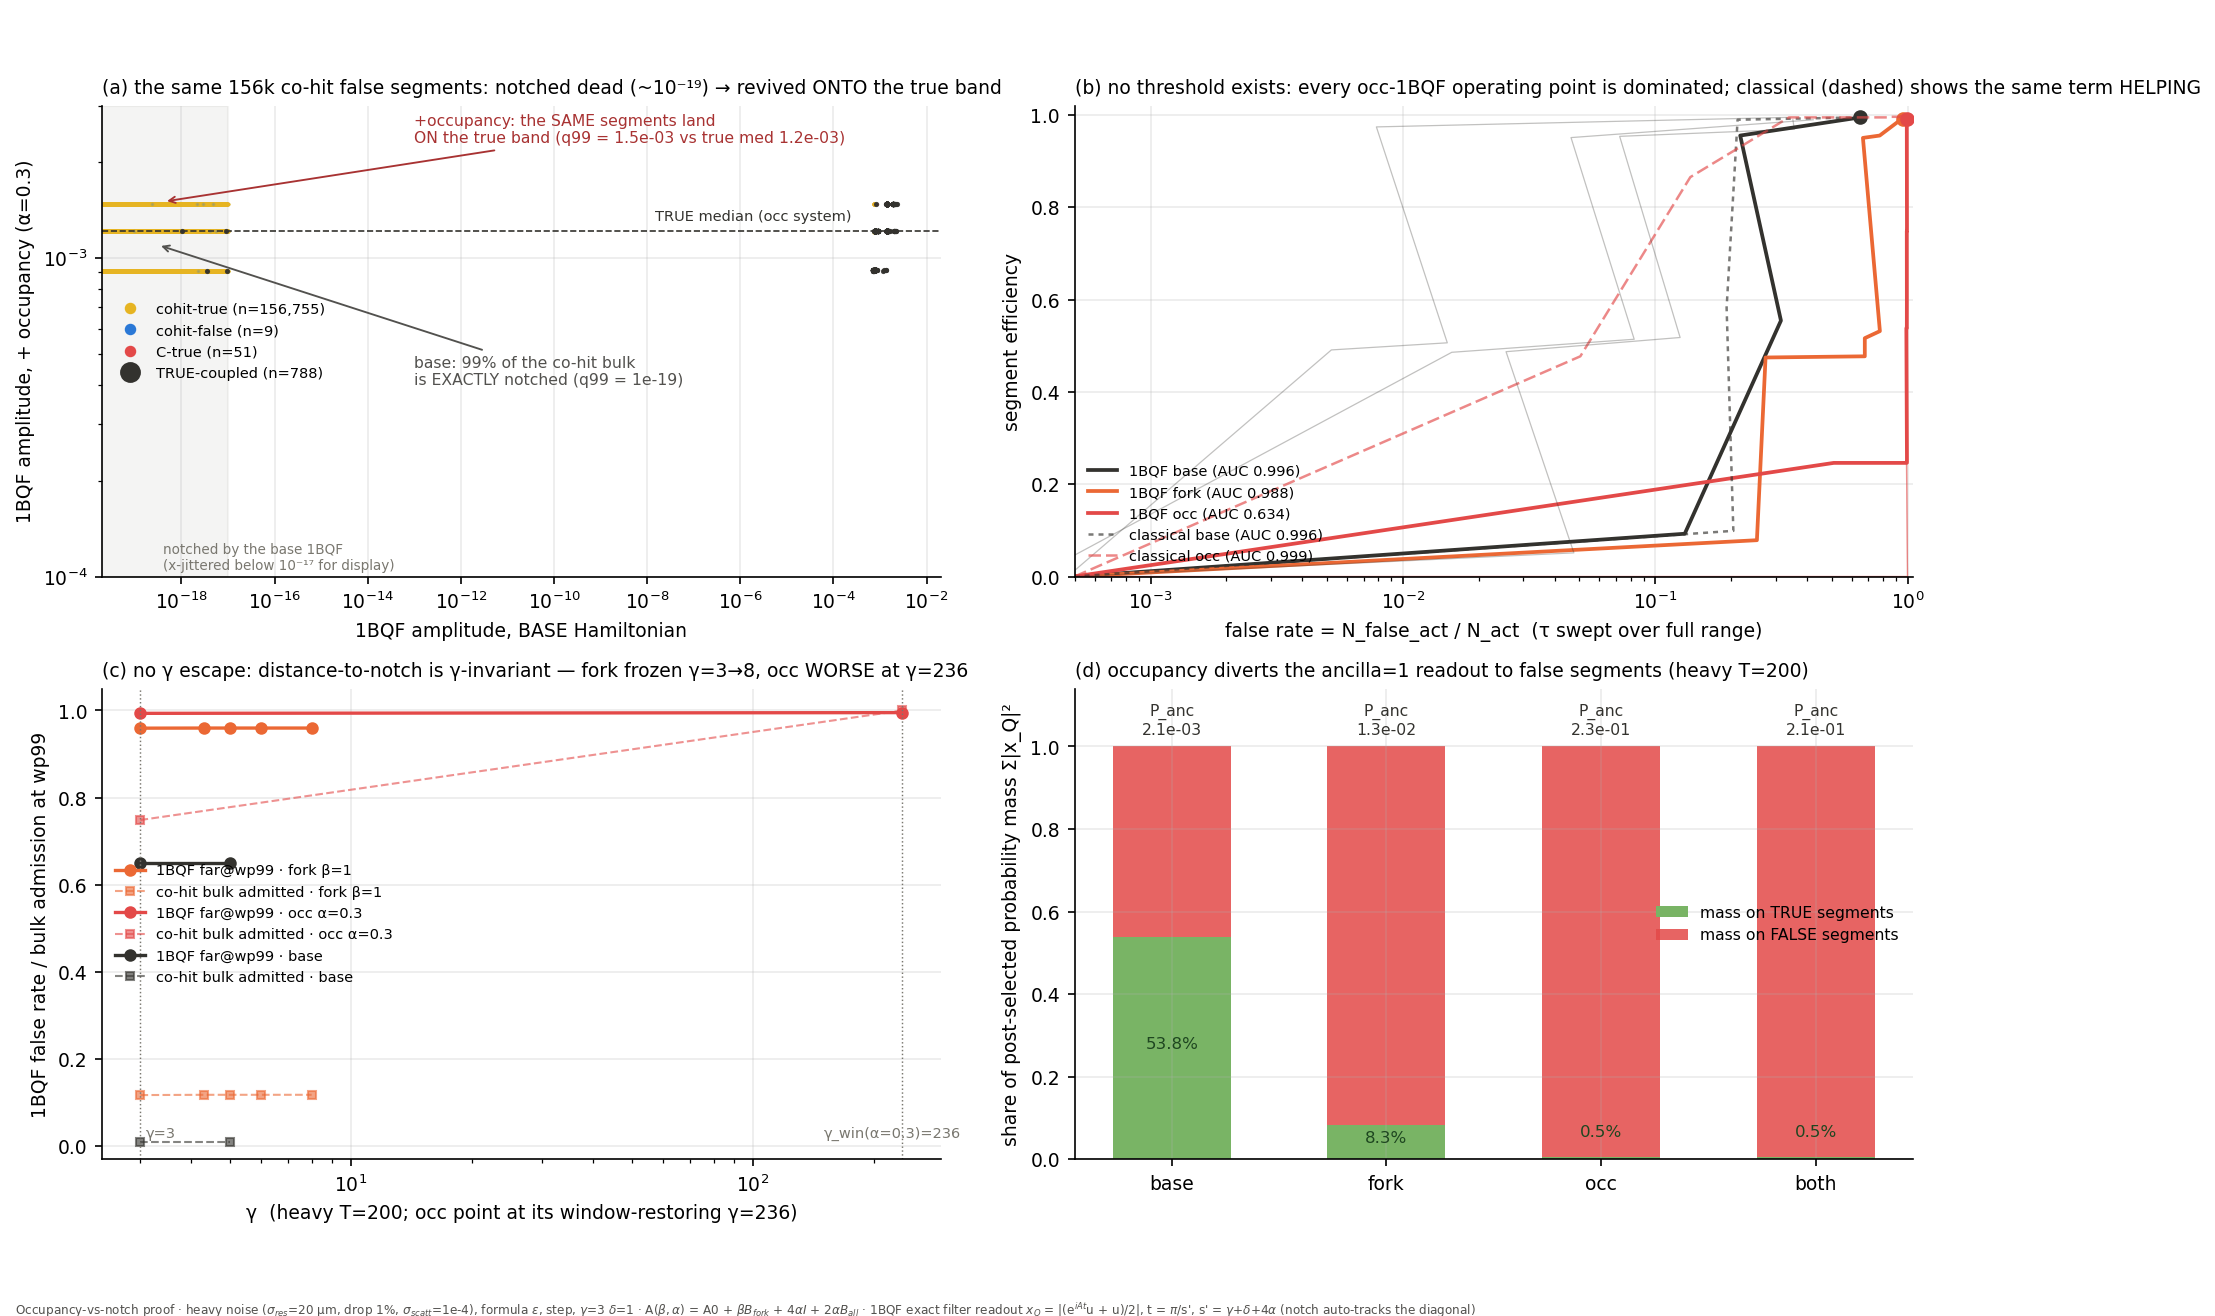
\includegraphics[width=0.95\textwidth]{dp_occupancy_proof.png}
\caption{The occupancy proof (heavy $T=200$): (a) the same co-hit
false segments, exactly notched under the base Hamiltonian, re-emerge
on the true amplitude band under $A_{\rm occ}$; (b) no threshold
escape: every occupancy-1BQF operating point is dominated, while the
same term helps the classical solver; (c) no $\gamma$ escape; (d) the
post-selected probability mass diverts to false segments.}
\label{fig:occproof}
\end{figure}

The mechanism generalises to any \emph{fixed} response: a spectral
filter earns its living from populations pinned to known eigenvalues,
and any Hamiltonian term that couples a pinned population unpins it.
For the 1BQF the verdict really is final, because the notch has no
further freedom to spend: its response family is exhausted by the
single parameter $t$, the retune $t=\pi/s'$ is already included
above, and figure~\ref{fig:occproof}(c) shows the $\gamma$ direction
offers no escape either. As a Hamiltonian term, occupancy is poison
to a notch, and the classical intuition for the term does not
transfer to it.\footnote{The occupancy constraint can also be applied
entirely outside the Hamiltonian, as a classical hit-uniqueness
post-selection applied evenly to every solver's output, deliberately kept out of this
work, whose subject is the spectral side.} But ``final for the
notch'' is not ``final for the filter family''. The fork term in the
next section will teach the general lesson of this paper, that an
operator modification can only be judged together with a response
refitted to the spectrum it creates, and
section~\ref{sec:fit:occ} returns to the occupancy term with exactly
that machinery. The verdict there reverses: what destroys the
degree-one filter turns out to be the single most helpful operator
modification in the study once the polynomial is allowed to follow
it.

% ══════════════════════════════════════════════════════════════════════════════
\section{The fork term and the moving spectrum}
\label{sec:fork}

\subsection{The term and its validity envelope}

The second Denby--Peterson penalty targets \emph{bifurcations}: two
segments claiming the same hit in the same role at small mutual
angle, the fork topology that produces the closely-competing
candidates a wide acceptance admits. The $\varepsilon$-windowed form
adds
\begin{equation}
A'=A+\beta\,B_{\rm fork}(\varepsilon_B),
\label{eq:fork}
\end{equation}
where $B_{\rm fork}$ couples co-hit same-role pairs within angular
window $\varepsilon_B$ (default: the acceptance itself). Unlike the
occupancy term, the fork is surgical where it matters. On clean
events it touches $\approx2\%$ of segments, and provably no
pure-true chain carries a fork edge, so the true comb lines are
$\beta$-invariant. Earlier classical-side work in this programme
established that the fork migrates contaminated-true spectral weight
back toward the comb bands; whether real solvers can collect that
migration is settled in section~\ref{sec:fit}.

Adding a positive semi-definite coupling widens the spectrum, and
the solver imposes two validity conditions with closed forms.
Positive definiteness requires $\gamma>\gamma_{\rm pd}=\gamma_{\rm
ref}-\lambda_{\min}$; the one-period condition of any cosine-family
filter (the top of the spectrum must not alias through the response
period) requires $\gamma>\gamma_{\rm win}=\lambda_{\max}-\gamma_{\rm
ref}-2\delta$, both extremes measured at a reference
$\gamma_{\rm ref}$ and shifted rigidly, since $\gamma$ enters only
the diagonal. At heavy $T=200$ the measured requirement is
$\gamma^*\approx3.4$ at $\beta=0.5$ and $\approx4.4$ at $\beta=1$.
The notch tracks the diagonal automatically ($t=\pi/s'$,
$s'=\gamma+\delta$), and the comb is rebuilt on the measured shifted
spectrum. Every fork result below carries these retunes; a
window-violating control ($\beta=0.5$ at $\gamma=3$) is kept in the
study to show they matter.

\subsection{The operator and the response are one design}
\label{sec:fork:nogo}

One methodological point, learnt the hard way, belongs here rather
than in a results table. Retuning a \emph{fixed} response to the fork
system --- tracking the diagonal, rebuilding the comb on the shifted
domain --- is not enough, because the retunes move the response's
centre and domain but never ask where the false weight now lives.
Evaluated that way, both Denby--Peterson terms read as regressions,
and the reading is a statement about the mismatch between an old
response and a new spectrum, not about the terms. The correct
procedure, used for every operator result in this paper, is to
measure the modified system's false pile-up and refit the polynomial
to it: change the Hamiltonian, and the activations and their spectral
support move; when they move, the polynomial must be refitted to the
moved spectrum. Carrying out that refit, for the fork and then for
the occupancy term, is the subject of section~\ref{sec:fit}. (A
second, smaller point: at heavy noise the efficiency-first convention
degenerates for an unrefitted comb, whose contaminated-true
amplitudes collapse toward zero, so sections~\ref{sec:fit} onward
compare solvers at matched efficiency instead.)

\subsection{A Trotter aside that will matter on hardware}
\label{sec:fork:trotter}

Everything in this paper so far treats the evolution $e^{iAt}$ as
exact. On hardware it is not: a quantum computer realises $e^{iAt}$
by a circuit, and the standard cheap construction, the
\emph{product formula} (or Trotterization), builds it from the
pairwise pieces of the Hamiltonian. The idea is simple: $A$ is a sum
of many small commuting-or-not terms, one per coupled segment pair,
and while $e^{i(X+Y)t}$ is hard, the product
$e^{iXt}e^{iYt}$ is easy --- one small gate per term. If $X$ and $Y$
commute the product is exact; if not, it errs at order $t^2[X,Y]$,
and one hopes the accumulated error stays below the physics. The
1BQF circuit of ref.~\cite{trackhhl} is exactly such a per-pair
product.

The programme's measurements show where that hope holds and where it
breaks, and the split is clean (figure~\ref{fig:erf}). With
\emph{uniform} coupling weights (every term the same strength, as in
the step-kernel Hamiltonian of this paper) circuit and exact
evolution agree to cosine similarity $\approx0.985$: the product
formula is safe. With \emph{heterogeneous} weights (the erf-weighted
angular kernel, or a fractional fork $\beta=0.5$ riding on unit
compatibility edges) the per-pair product scatters the readout badly
enough to dominate the physics: on the fork system the circuit reads
false rate $0.96$ where the exact evolution reads $0.73$, and on the
erf kernel removing the product formula alone collapses the false
rate from $0.83$ to $0.22$ at moderate noise. The rule of thumb for
hardware is that heterogeneous coupling weights break the naive
product formula, and circuit realisations of weighted Hamiltonians
need the structured synthesis route (edge-coloured pair ordering)
developed in the programme's direct-structural-synthesis study. All
fork and fit results in this paper use exact evolution precisely so
that filter physics and circuit error are never conflated;
section~\ref{sec:limits:trotter} returns to what this means for
deployment.

\begin{figure}[t]
\centering
\captionsetup{width=0.92\textwidth}
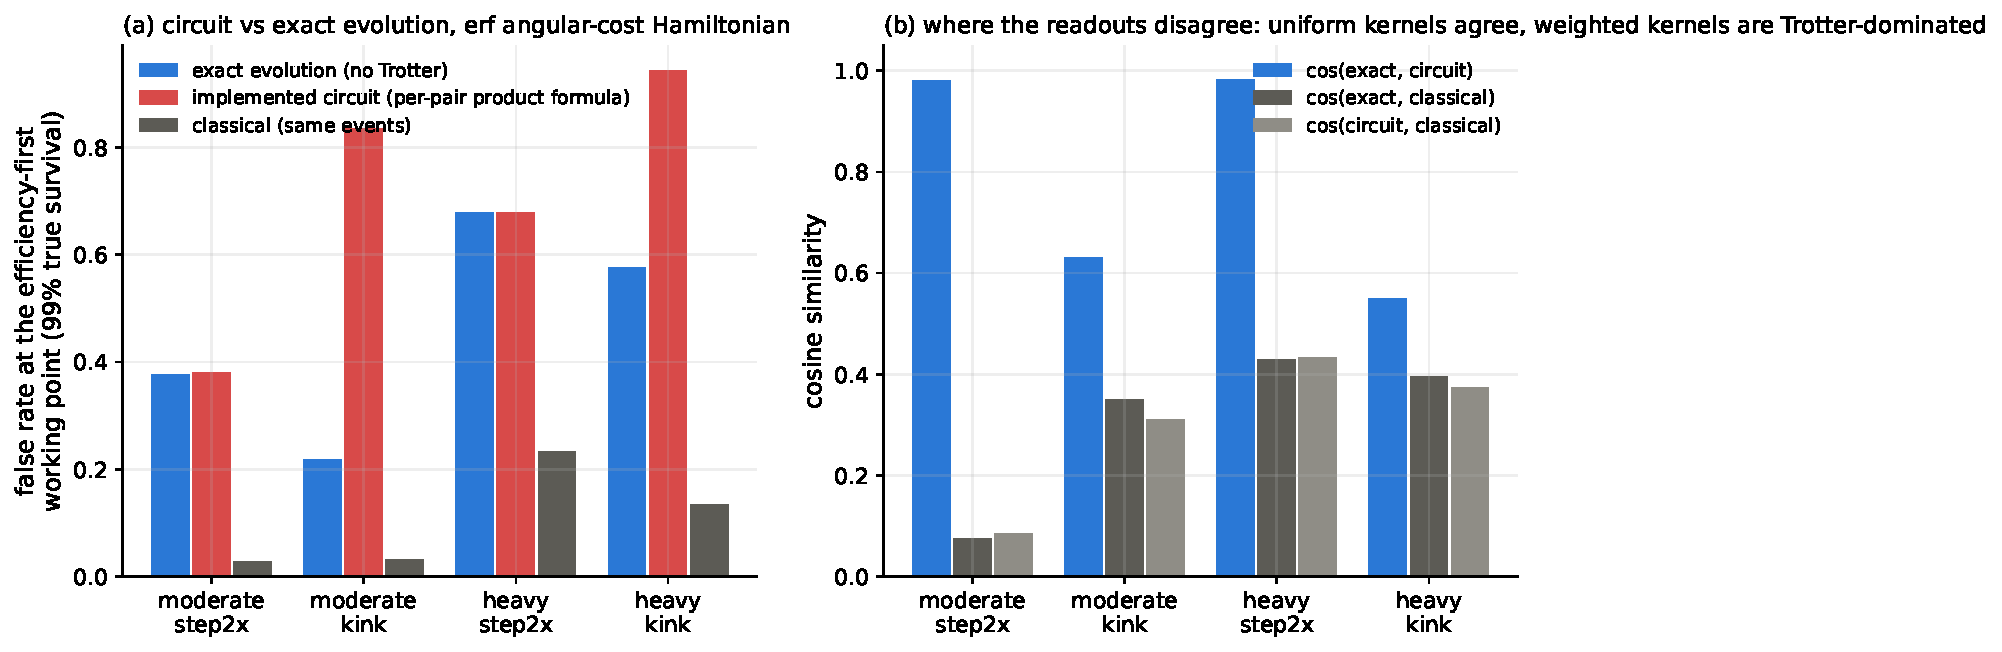
\includegraphics[width=0.95\textwidth]{erf_exact_evolution_paper.pdf}
\caption{The exact-evolution arbiter on the erf angular-cost
Hamiltonian (heavy and moderate noise, $T=200$). (a) False rate at
the efficiency-first working point: exact evolution against the
implemented product-formula circuit and the classical baseline on
the same events. Uniform-weight kernels (step2x) show circuit $=$
exact, so the remaining deficit is physics; weighted kernels (kink)
are Trotter-dominated. (b) The same story as readout fidelity:
cosine similarity between the three solutions.}
\label{fig:erf}
\end{figure}

% ══════════════════════════════════════════════════════════════════════════════
\section{Fitting the polynomial to noisy events: roots at the
measured pile-up}
\label{sec:fit}

\subsection{Measuring the false pile-up}

The fit begins with a measurement no fixed design ever asked for:
where, exactly, does the false amplitude come from? Because
the heavy-noise compatibility graph has no giant component
(section~\ref{sec:noise}), the per-component eigendecomposition
gives, for every eigenvalue in the event, its exact content: how
much of the mode's weight lies on true segments, how much on false,
and how much of each segment's amplitude it builds. Under any
response $p$,
\begin{equation}
x_s(p)=\sum_i p(\lambda_i)\,\big(\mathbf{v}_i^{\!\top}\mathbf{b}\big)\,
v_i(s),
\label{eq:linresponse}
\end{equation}
linear in $p$, so the question of where the false amplitude comes
from is well posed and exactly answerable. The answer, on the heavy
$T=200$ events, is concentrated to a degree I did not expect. The
false-active formation weight piles up on the \emph{pair line}
$\lambda=s-1$: on the three events measured, that single bin carries
$1122$--$1378$ weight units against $4$--$10$ units of true weight,
with the triple lines $s\pm\sqrt2$ next; the overall bin-level
overlap between false-active and true formation is $0.014$--$0.023$
in cosine. The false population is not smeared. It is parked on the
eigenvalue lines of identifiable two- and three-segment motifs,
almost none of which are shared with true formation.

\subsection{Fitting the response}

With eq.~\eqref{eq:linresponse} linear in the response, the fit is a
regularised least-squares problem over binned response values
($\Delta\lambda=0.02$):
\begin{equation}
\min_{p}\ \sum_{s\,\in\,\rm false}x_s(p)^2
\;+\;\mu\sum_{s\,\in\,\rm true}\big(x_s(p)-x_s^{\rm cls}\big)^2 ,
\qquad |p|\le1,
\label{eq:fit}
\end{equation}
with the isolated-false line pressured to zero and $\mu$ swept to
trace the efficiency--purity trade. No root position is chosen by
hand: zeros appear where false weight concentrates because that is
what the objective rewards. The fitted response reproduces the
comb's passes at the (contamination-shifted) true lines and drives
deep roots through $s-1$ and $s\pm\sqrt2$: precisely the polynomial
that no clean-event design could have anticipated, because the root
locations are properties of the measured noise.

\subsection{Results}
\label{sec:fit:results}

Table~\ref{tab:fit} is the main result of the section, and it is
worth being explicit about how to read it, because every number in
it is the same kind of object. Fix a system (a row block: the base
Hamiltonian, or the fork system at its validity point) and a target
efficiency (the ``eff'' column). For each solver, slide that
solver's own threshold until exactly the target fraction of true
segments survives --- the matched-efficiency convention of
section~\ref{sec:toy:metrics} --- and record the false rate of the
selected sample at that threshold. Lower is better; solvers in the
same row are compared at identical efficiency by construction, so
the false rate is the \emph{entire} difference between them. All
numbers are means over three events, heavy noise, $T=200$.

\begin{figure}[t]
\centering
\captionsetup{width=0.93\textwidth}
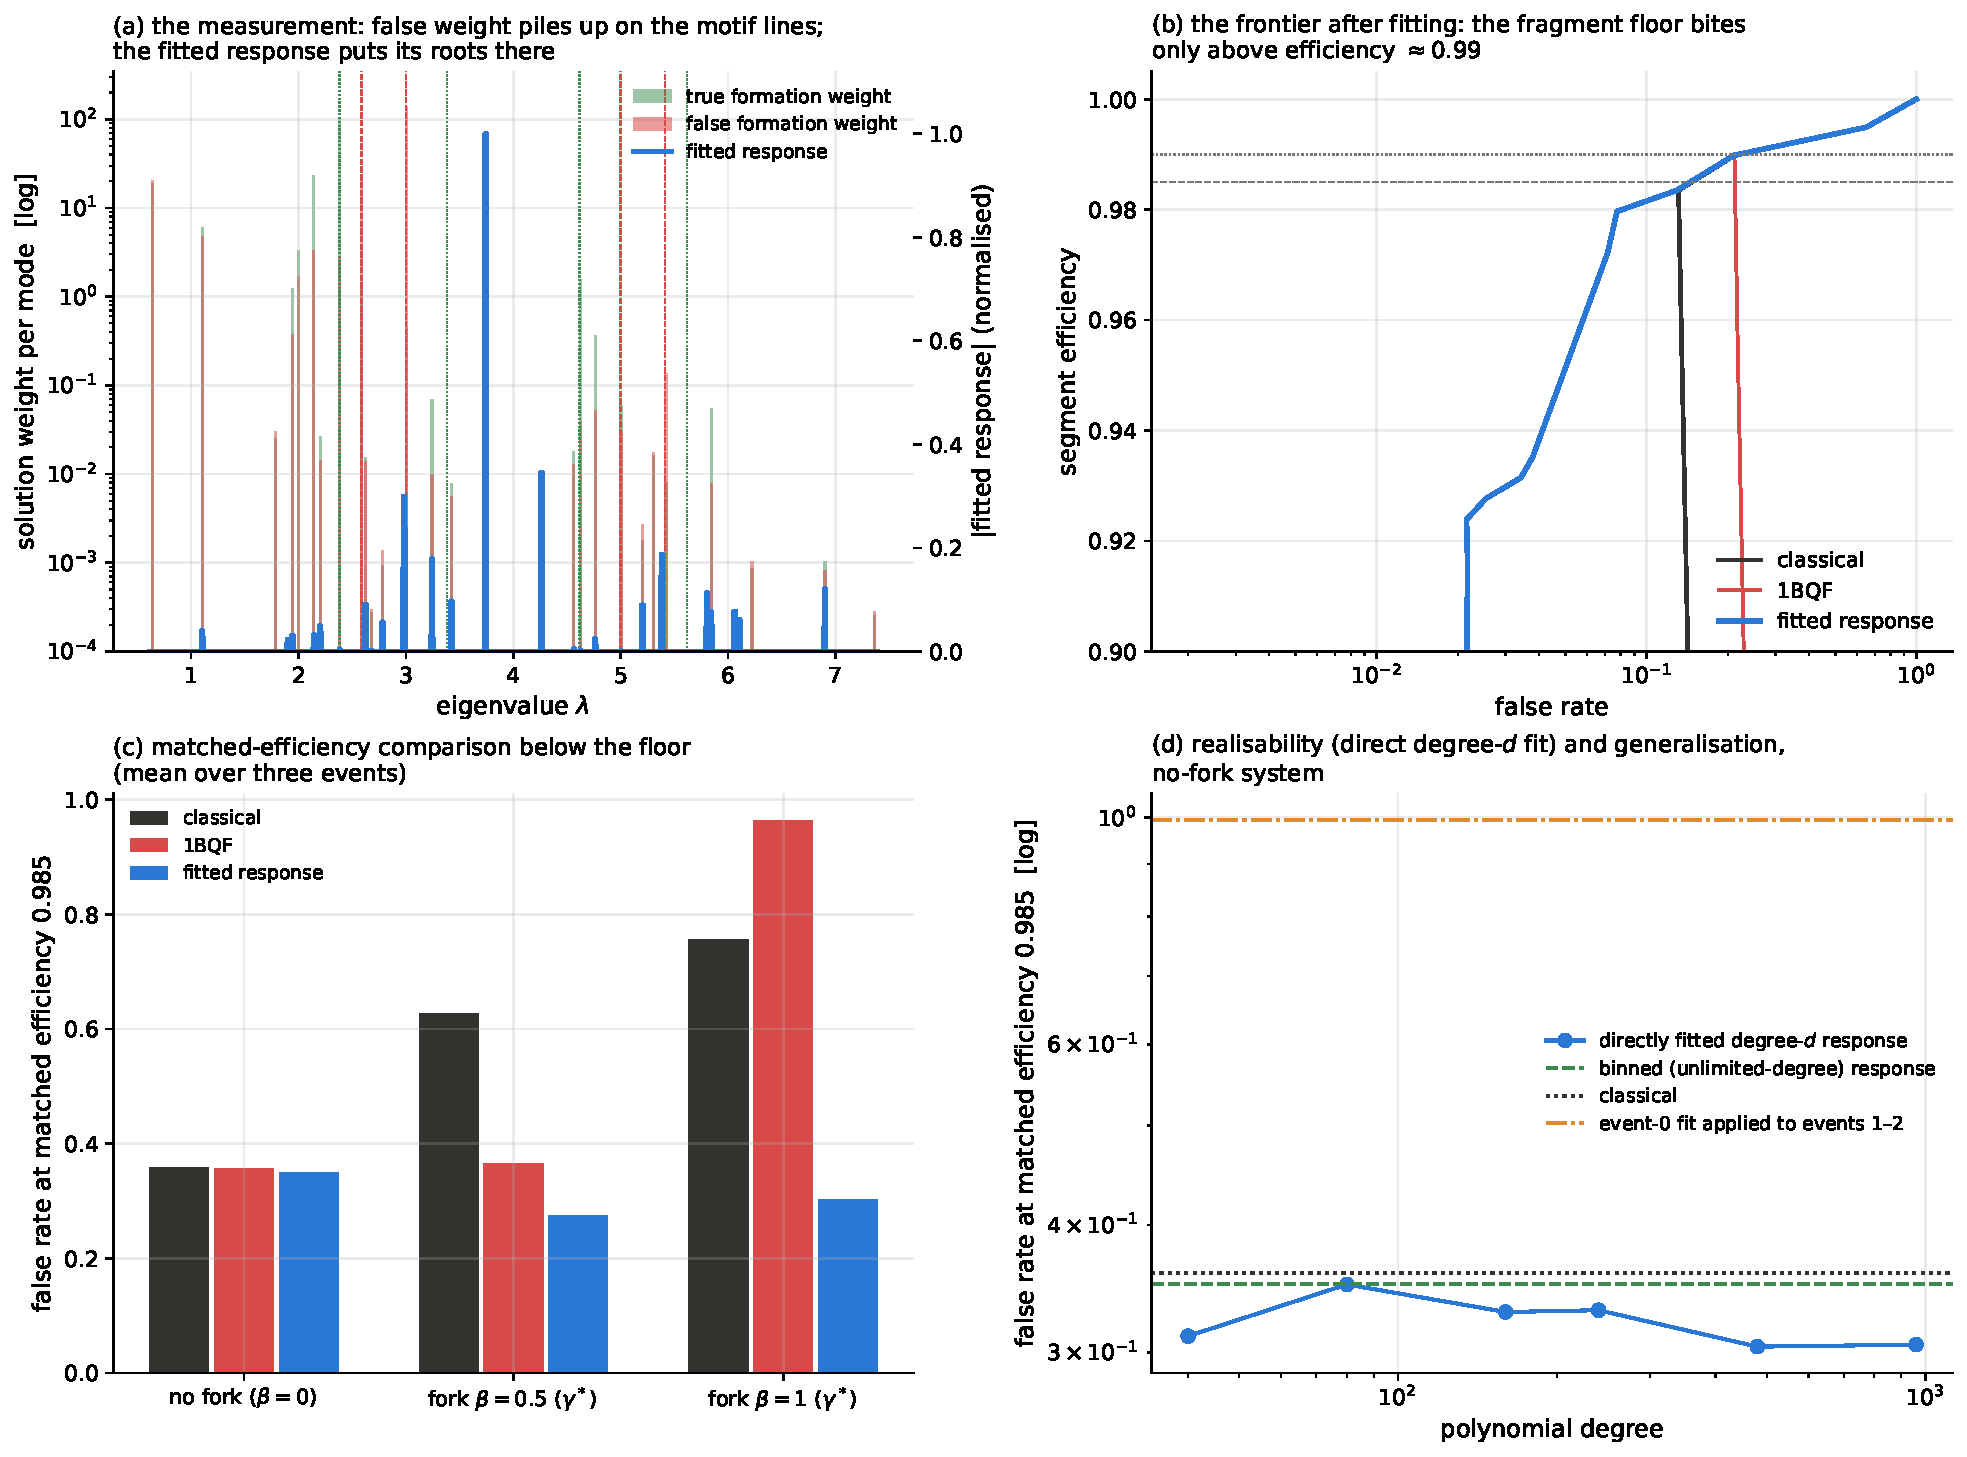
\includegraphics[width=0.98\textwidth]{fit_comb_paper.pdf}
\caption{Fitting the response to the measured pile-up (heavy
$T=200$): (a) exact per-mode false (red) and true (green) formation
weight against $\lambda$, with the fitted response overlaid; the
fitted roots land on the pair and triple lines. (b) The resulting
efficiency/false-rate frontier, with the fragment floor biting
only above $\eff\approx0.99$. (c) False rate at matched efficiency
$0.985$ for the base and fork systems (three-event means). (d) The
same quantity for responses fitted directly at fixed polynomial
degree: production-scale degrees already realise the measured
optimum (section~\ref{sec:limits:realizability}).}
\label{fig:fit}
\end{figure}

\begin{table}[H]
\centering
\begin{tabular}{llccc}
\toprule
system & eff & classical & 1BQF & \textbf{fitted response}\\
\midrule
base ($\beta=0$)        & 0.98 & 0.124 & 0.199 & \textbf{0.096}\\
base ($\beta=0$)        & 0.97 & 0.124 & 0.199 & \textbf{0.061}\\
fork ($\beta=0.5,\gamma^*$) & 0.98 & 0.463 & 0.145 & \textbf{0.085}\\
fork ($\beta=0.5,\gamma^*$) & 0.97 & 0.292 & 0.124 & \textbf{0.046}\\
\midrule
either              & 0.99 & 0.63--0.76 & 0.65--0.96 & 0.63--0.77\\
\bottomrule
\end{tabular}
\caption{Segment false rate at matched efficiency (lower is better):
each solver's threshold is set so the stated fraction of true
segments survives, and the false rate of the resulting selection is
quoted. Heavy noise, $T=200$, three-event means. ``Fitted response''
is the optimal binned response of eq.~\eqref{eq:fit}, refitted to
each system. The last row is the fragment floor of
section~\ref{sec:fit:floor}: at $\eff=0.99$ every solver floods, on
the base and fork systems alike.}
\label{tab:fit}
\end{table}

Three conclusions follow.

First, the expected ordering is restored. Below efficiency
$\approx0.985$ the fitted quantum filter sits under the classical
baseline everywhere: $0.096$ against $0.124$ at $\eff=0.98$, $0.061$
against $0.124$ at $\eff=0.97$. The claim this section set out to
test, that the false rate should still be lower for the quantum
filters once they are fitted, holds.

Second, the fork earns its keep, but only through the refit. On the
fork system the fitted response
reaches $0.046$ at $\eff=0.97$, beating the fitted no-fork system's
$0.061$, while the classical solver on the same fork system reads
$0.292$. The operator knob does exactly what the spectral-migration
analysis promised, provided the response follows it: changing the
Hamiltonian without refitting the polynomial is not a half-measure,
it is worse than doing neither
(section~\ref{sec:fork:nogo}). The standard-notch 1BQF also benefits
from the fork
below the floor ($0.145$ against $0.199$ at $\eff=0.98$): the fork
pushes coupled-false modes away from the passband even when the
only zero sits at $s'$.

Third, the wall at $\eff\ge0.99$ is real on these systems, and now
has a name. At the strict $99\%$ point everything, classical
included, floods back to $\far\approx0.65$. The per-component
decomposition locates the cause exactly: about $2\%$ of \emph{true}
segments --- a couple of dozen per event, counted directly and
consistently on all three events --- are spectral twins of the false
motifs, in exactly the sense of
section~\ref{sec:comb:limits} and figure~\ref{fig:twins}. They are
the hit-drop fragments of section~\ref{sec:comb:drop}: a broken
track's two-segment piece \emph{is} a pair, sitting on the pair
line, in a pure-true component, plus a handful of contaminated mixed
chains. Any response with a root at $s-1$ kills them alongside the
false pairs; their population exceeds the $1\%$ efficiency budget;
and once the working point must dip below their suppressed
amplitudes, the entire suppressed false band comes back above
threshold. This is the \emph{fragment floor}: the noisy-event
generalisation of the clean floor theorem, no longer a curiosity but
the binding constraint. The robust statement is the measured wall
itself: on the base and fork systems every solver holds
$\eff=0.98$ and none holds $\eff=0.99$, on all three events. On
\emph{those} Hamiltonians no function of $\lambda$ can cross it ---
but the floor is a twin degeneracy of the operator, not of the
event, and the next subsection shows an operator that removes it.
\label{sec:fit:floor}

\subsection{The occupancy term, refitted}
\label{sec:fit:occ}

Section~\ref{sec:occupancy} ended with a debt: the occupancy was measured on the fixed 1BQF targeting the central, isolated, eigenvalue, a filter with no freedom to follow the
spectrum the term creates, and the fork has since taught us that
operator terms can only be judged with a refitted response. The
occupancy system makes the refit technically harder --- the co-hit
coupling $2\alpha B_{\rm all}$ merges the compatibility graph into a
giant component, so the exact per-component measurement behind
eq.~\eqref{eq:fit} is unavailable --- but not impossible: a degree-$d$
response needs no eigendecomposition, because the moment vectors
$T_k(X)\mathbf{b}$ are computable by sparse matrix--vector recursion
and the amplitudes are linear in the Chebyshev coefficients. The fit
of eq.~\eqref{eq:fit} then becomes an exact least-squares problem in
$d{+}1$ coefficients, over \emph{every} segment of the event
including the isolated bulk. Run identically on the base and
occupancy systems (same algorithms, same events, only the Hamiltonian
differs), it settles the question.

The verdict of section~\ref{sec:occupancy} reverses
(figure~\ref{fig:occfit}). At matched efficiency $0.98$ the directly
fitted response reads $0.085$ on the base system and $0.050$ on the
occupancy system at $\alpha=0.05$; at $0.97$, $0.071$ against
$0.039$. The term that destroys the notch roughly halves the false
rate of the fitted polynomial, while the classical solver on the
same systems sits at $0.12$ throughout. Two structural findings come
with the headline. First, \emph{small coupling wins}:
$\alpha=0.05$ beats the classically-motivated $\alpha=0.3$
($0.050$ vs $0.067$ at matched efficiency $0.98$), because the
occupancy term stretches the spectral span ($6.7\to43\to242$ for
$\alpha=0\to0.05\to0.3$) and a fixed degree budget loses resolution
proportionally; the spectral benefit saturates long before the
classical amplitude benefit does. Second, and most strikingly,
\emph{the occupancy coupling breaks the fragment floor}. One of the
three events is floor-bound on the base system --- its fitted
response cannot do better than $0.654$ at matched efficiency
$0.985$, because its fragment twins are exactly degenerate with
false pairs --- and on the occupancy system the same event fits to
$0.062$. The mechanism is the floor theorem read in reverse: the
twin argument requires isomorphic components, and the co-hit
coupling embeds every motif in its hit-sharing neighbourhood, which
is different for a fragment of a real track than for an accidental
false pair. The embedding breaks the isomorphism, the degeneracy
lifts, and a response fitted to the new spectrum separates what was
provably inseparable on the base Hamiltonian. The fragment floor of
section~\ref{sec:fit:floor} is therefore a property of the
\emph{base} Hamiltonian, not of the problem.

One engineering note: the degree budget
that collects the occupancy win is larger than the base system's
(the span costs resolution; most of the gain arrives by degree
$80$--$160$ at $\alpha=0.05$). Like every fitted result in this
section, the fit itself is mechanical --- the roots land on the
enumerable motif structure the operator produces --- so the reversal
is a property of the Hamiltonian, not of a tuning; folding it into
the single fixed response of
section~\ref{sec:limits:generalization} is part of that
enumeration.

\begin{figure}[t]
\centering
\captionsetup{width=0.92\textwidth}
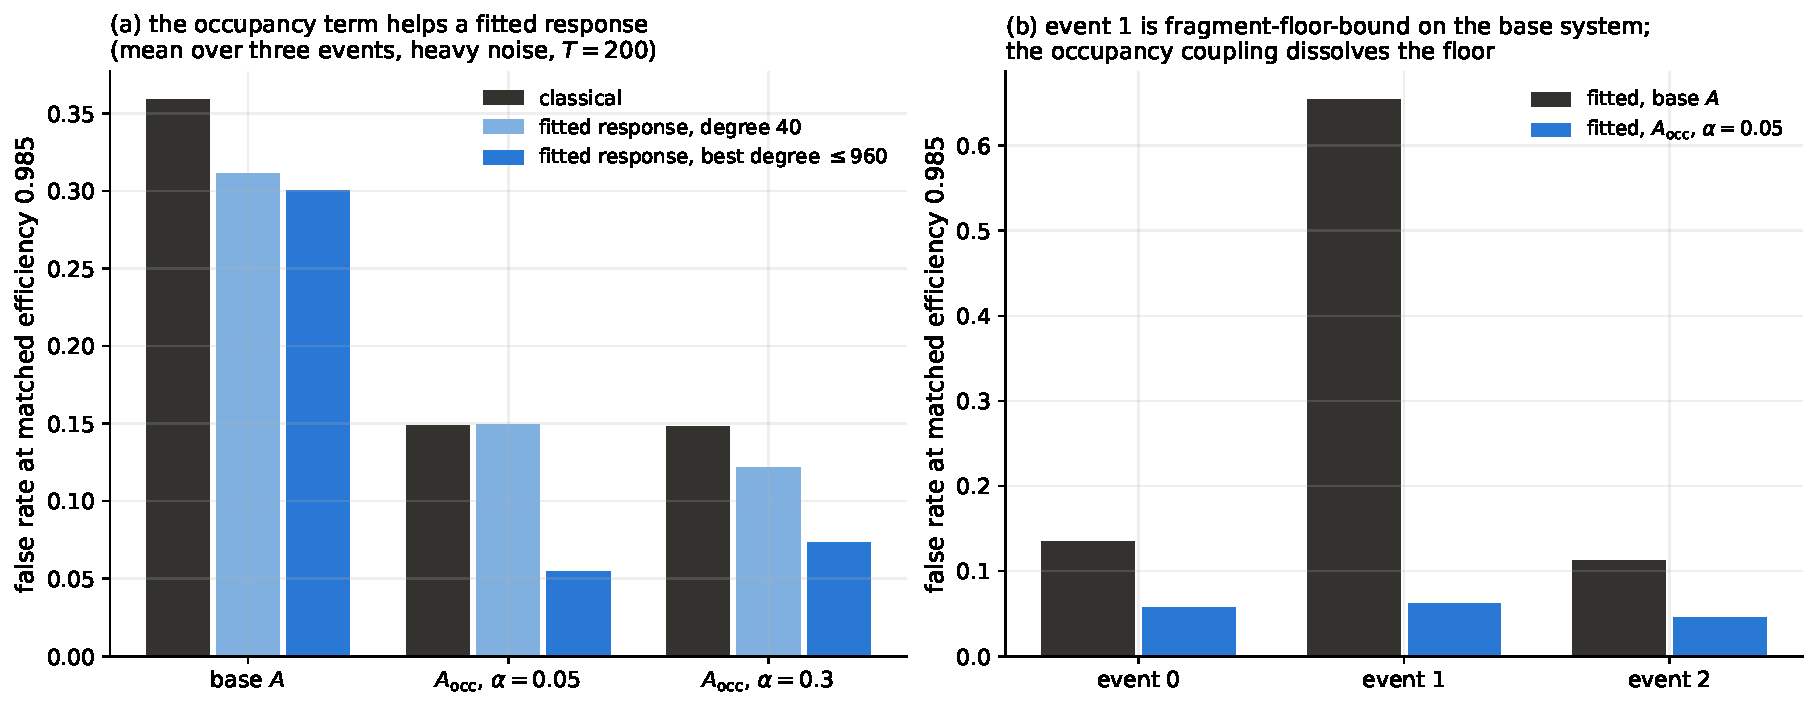
\includegraphics[width=0.95\textwidth]{occupancy_fitted.pdf}
\caption{The occupancy term, refitted (heavy $T=200$, degree-$d$
responses fitted directly in coefficient space; identical machinery
on every system). (a) False rate at matched efficiency $0.985$,
three-event means: the fitted response on the occupancy system at
$\alpha=0.05$ beats both the classical solver and the fitted
response on the base system. (b) Per event: the event that is
fragment-floor-bound on the base system (event 1) escapes the floor
on the occupancy system --- the co-hit coupling breaks the
fragment/false-pair twin degeneracy.}
\label{fig:occfit}
\end{figure}

\subsection{Why the 1BQF specifically cannot follow}
\label{sec:fit:rootbudget}

A degree-one filter owns one zero, and the measurement says the
heavy false spectrum has two mandatory root locations: the isolated
line at $s$ ($\mathcal{O}(10^5)$ segments) and the pair line at
$s-1$ (the active pile-up). The study's control makes the conflict
vivid. Retuning the notch onto the pair line ($t=\pi/(s{-}1)$) does
root the pile-up, and releases the isolated bulk, which re-enters
at amplitude $|\cos(st/2)|\,\delta=0.5$, on top of the true band,
for a false rate of $0.995$. The 1BQF's zero is spoken for.
Covering both lines is degree two; covering the triple lines as
well is degree four and up; and that, stated as a root budget, is
in my opinion the cleanest justification for the whole QSVT
programme that the toy has produced.

% ══════════════════════════════════════════════════════════════════════════════
\section{Limitations}
\label{sec:limits}

I collect here, deliberately and in one place, everything that
stands between the results above and a deployable algorithm. Each
limitation comes with its measured size and, where we have one, its
escape route.

\subsection{Realizability of the fitted response}
\label{sec:limits:realizability}

An earlier version of this study believed realizability was the
bottleneck, and the false alarm is worth recording because the
resolution strengthens the result. The binned optimum of
eq.~\eqref{eq:fit} has features of width $\approx0.02$ on a spectral
span of $\approx7$; a Chebyshev series \emph{reproducing that
specific function} needs degree $d\approx2W/h\approx700$, and truncated
series fitted to it at $d\le240$ performed terribly. But reproducing
the binned optimum is the wrong problem. Fitting the objective of
eq.~\eqref{eq:fit} \emph{directly in the degree-$d$ coefficient
space} --- amplitudes are linear in the Chebyshev coefficients, so
this is the same least-squares problem in $d{+}1$ unknowns --- finds
realisable responses that match the unlimited-degree optimum already
at the production degree
(figure~\ref{fig:fit}d: $0.099$ at $d=40$ against the binned
optimum's $0.096$ at matched efficiency $0.98$ on the base system).
The measured discrimination of section~\ref{sec:fit} is therefore
available at circuit-affordable degree; nothing about the polynomial
family was ever in the way, only the indirect two-step fit.

A structural escape remains available on top: the same
no-giant-component fact that made the spectrum measurable makes the
problem block-diagonal. Solving
per connected component (a classical $\mathcal{O}(n)$ preprocessing
step) replaces one $4T^2$-dimensional filter problem by hundreds of
$\le17$-dimensional ones, on which a degree-$\le17$ interpolating
polynomial reproduces any response exactly, and as a bonus the
register shrinks to $\lceil\log_2 17\rceil+2$ qubits and the
success probability per cluster becomes $\mathcal{O}(1)$. The cost
is honesty about what remains quantum: per-cluster solving helps
the classical solver identically, and the quantum claim reduces to
the resource profile of section~\ref{sec:qsvt:resources} on
whatever cluster sizes survive preprocessing.

\subsection{One response for all events}
\label{sec:limits:generalization}

On this toy the fit is not a statistical learning problem, and no
train-and-test machinery is needed to understand it. The structures
an event can contain are enumerable --- chains, hubs, bridges and
their contaminated combinations, each pinned to closed-form
eigenvalue lines --- and the fit is mechanical: the roots land on
the motif lines because that is where the false weight must sit.
The root positions are therefore universal ($s-1$ and $s\pm\sqrt2$
are motif properties, not event properties). What does vary between
events is the contaminated-true pass positions, which chase each
noise realisation's particular contaminated modes: a response taken
verbatim from one event and applied to another reads $0.63$--$0.99$
false rate against $0.04$--$0.10$ on its own event, entirely
because its narrow passes sit at the wrong contaminated positions.
A production design is then an enumeration exercise, not a fitting
one: roots pinned to the motif lines, passes wide enough to cover
the contaminated-true spread of the ensemble. Building that single
fixed response, and measuring what its wider passes cost against
the per-event ceiling of section~\ref{sec:fit}, is the programme's
clear next step. On noisier data --- real geometry, variable track
length, denser contamination --- the structure will no longer be
enumerable by hand, and how to fix the response there will need
closer thought (section~\ref{sec:limits:geometry}).

\subsection{Trotterization on hardware}
\label{sec:limits:trotter}

Everything above uses exact evolution. On hardware, the 1BQF's
product-formula circuit is exact only in the uniform-coupling case;
the moment coupling weights differ (erf-weighted kernels,
fractional fork strengths) the naive per-pair formula scatters the
readout by amounts that dominate the physics
(section~\ref{sec:fork}). The structured-synthesis route
(edge-coloured pair ordering, developed in the programme's DSS
study, which also reaches 1BQF width for the comb via generalized
QSP over $e^{-iAt}$) restores exactness at matched cost and is, on
present evidence, mandatory for any weighted Hamiltonian on
hardware.

\subsection{Success probability and readout}
\label{sec:limits:readout}

The filtered state must still be post-selected and read out, and it
is worth being explicit about what that costs, because it is the
largest single overhead in the whole scheme
(figure~\ref{fig:readout}). The LCU post-selection succeeds when the
index and dilation registers both return zero, which happens with
probability $P_{\rm anc}$ of eq.~\eqref{eq:psucc}; physically,
$P_{\rm anc}$ is the fraction of the input state's norm that
survives the filter. Because the uniform input spreads over all
$4T^2$ segments while only $\mathcal{O}(T)$ of them carry surviving
amplitude, $P_{\rm anc}$ falls as $1/T$: measured
$\approx0.44/T$ for the comb and estimated $\approx0.25/T$ for the
1BQF, i.e.\ thousandths at $T=1000$. Left alone this would mean
thousands of repetitions per useful sample. Amplitude amplification
(the standard Grover-type trick) reduces the repetition count from
$1/P_{\rm anc}$ to $1/\sqrt{P_{\rm anc}}$, restoring a $\sqrt T$
scaling of total walk calls per useful sample, and active-set
readout (sampling until the $\mathcal{O}(T)$ surviving segments are
each seen) gives the measured $d\cdot T^{1.5}\log T$ walk-call
budget against the classical $d\cdot T^{2}$ flop budget: a
square-root-class separation for that readout task, and no more
than that.

\begin{figure}[t]
\centering
\captionsetup{width=0.92\textwidth}
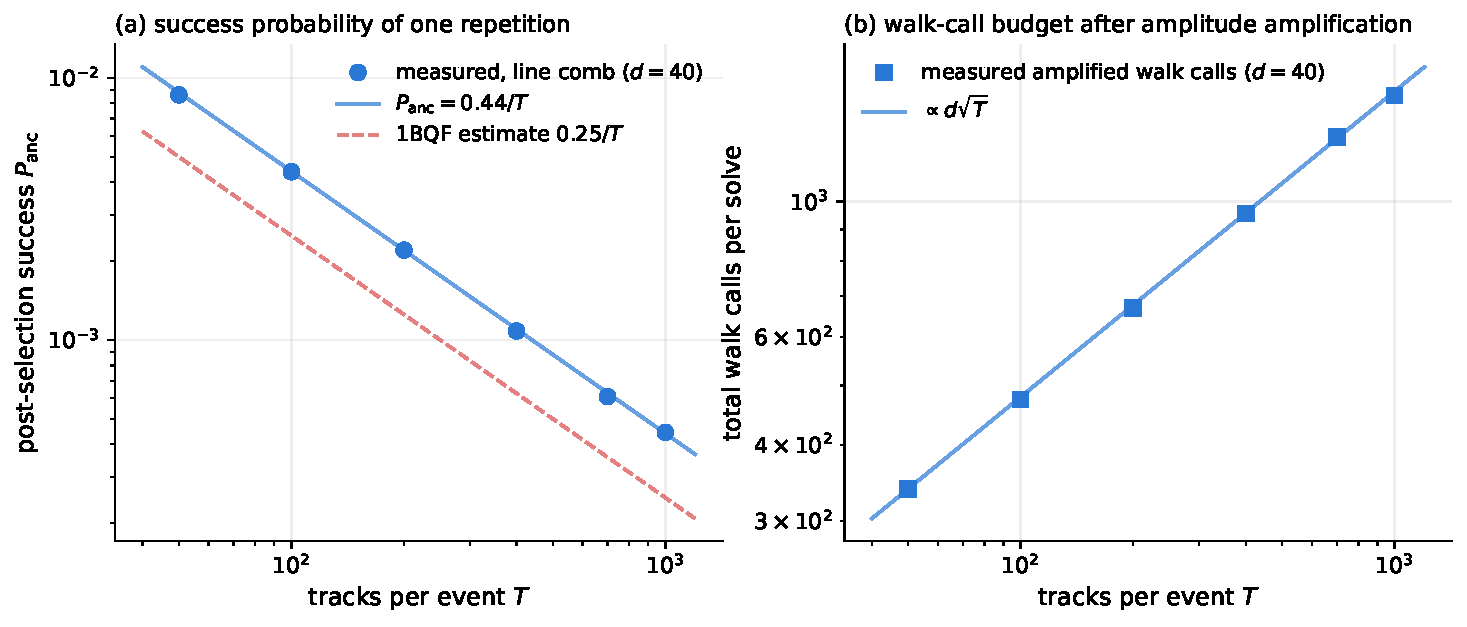
\includegraphics[width=0.95\textwidth]{readout_probability.pdf}
\caption{The readout budget, measured on the shared events at the
production degree $d=40$. (a) Post-selection success probability per
repetition: the measured comb points follow $0.44/T$; the 1BQF
estimate $0.25/T$ is shown for comparison. (b) Total walk calls per
solve after amplitude amplification, following the $d\sqrt T$
scaling.}
\label{fig:readout}
\end{figure}

\subsection{Classical simulability of the response family}
\label{sec:limits:dequant}

Every response function in this paper can be applied classically by
the Chebyshev recursion in $\mathcal{O}(d\cdot{\rm nnz}(A))$ flops,
seconds at $T=1000$. The discrimination physics (combs, roots,
floors) is solver-independent mathematics of the segment
Hamiltonian, and this paper's contribution to it stands whether or
not a quantum computer is ever involved. The quantum claim is
confined to the resource profile: width logarithmic in problem
size, walk calls $d\sqrt T$ against classical $dT^2$ for the
readout task above, and a hardware-native route to the same
amplitudes. Readers allergic to quantum advantage claims may read
the whole paper as classical spectral-filter engineering with a
quantum implementation appendix; nothing in the physics sections
would change.

\subsection{The toy's geometry, and what a real detector changes}
\label{sec:limits:geometry}

Finally, the largest caveat of all: the four-line comb exists
because this toy pins every true track to five hits. Real VELO
tracks have variable length, and a companion study on real Run-3
event geometry found the true spectrum smeared into a band, the
$P_4$ comb keeping only $40\%$ of true segments, and a
short-fragment floor ($m\le2$ tracks indistinguishable from noise
at the segment level) capping all segment-level solvers, while the
fork transfer and the band-plus-notch redesign behaved as the toy
predicts. Figure~\ref{fig:run3} shows the measured amplitude
pile-up on the real geometry, side by side for the three solver
designs: where the toy's amplitude atlas (figure~\ref{fig:atlas})
has discrete levels, the real geometry smears the true population
into a continuum, the fragment population ($m\le2$, orange) sits
inside the false bulk for every solver, and the redesigned
band-plus-notch response reproduces the toy's qualitative
separation on the findable ($m\ge3$) population. The honest
statement of scope is that this paper's method
is response engineering on whatever spectral structure the geometry
provides, demonstrated exhaustively on a geometry that provides a
lot of it; the measurement loop of section~\ref{sec:fit} (measure
the pile-up, fit the response, locate the floor) is
geometry-agnostic even where the specific comb is not.

\begin{figure}[t]
\centering
\captionsetup{width=0.95\textwidth}
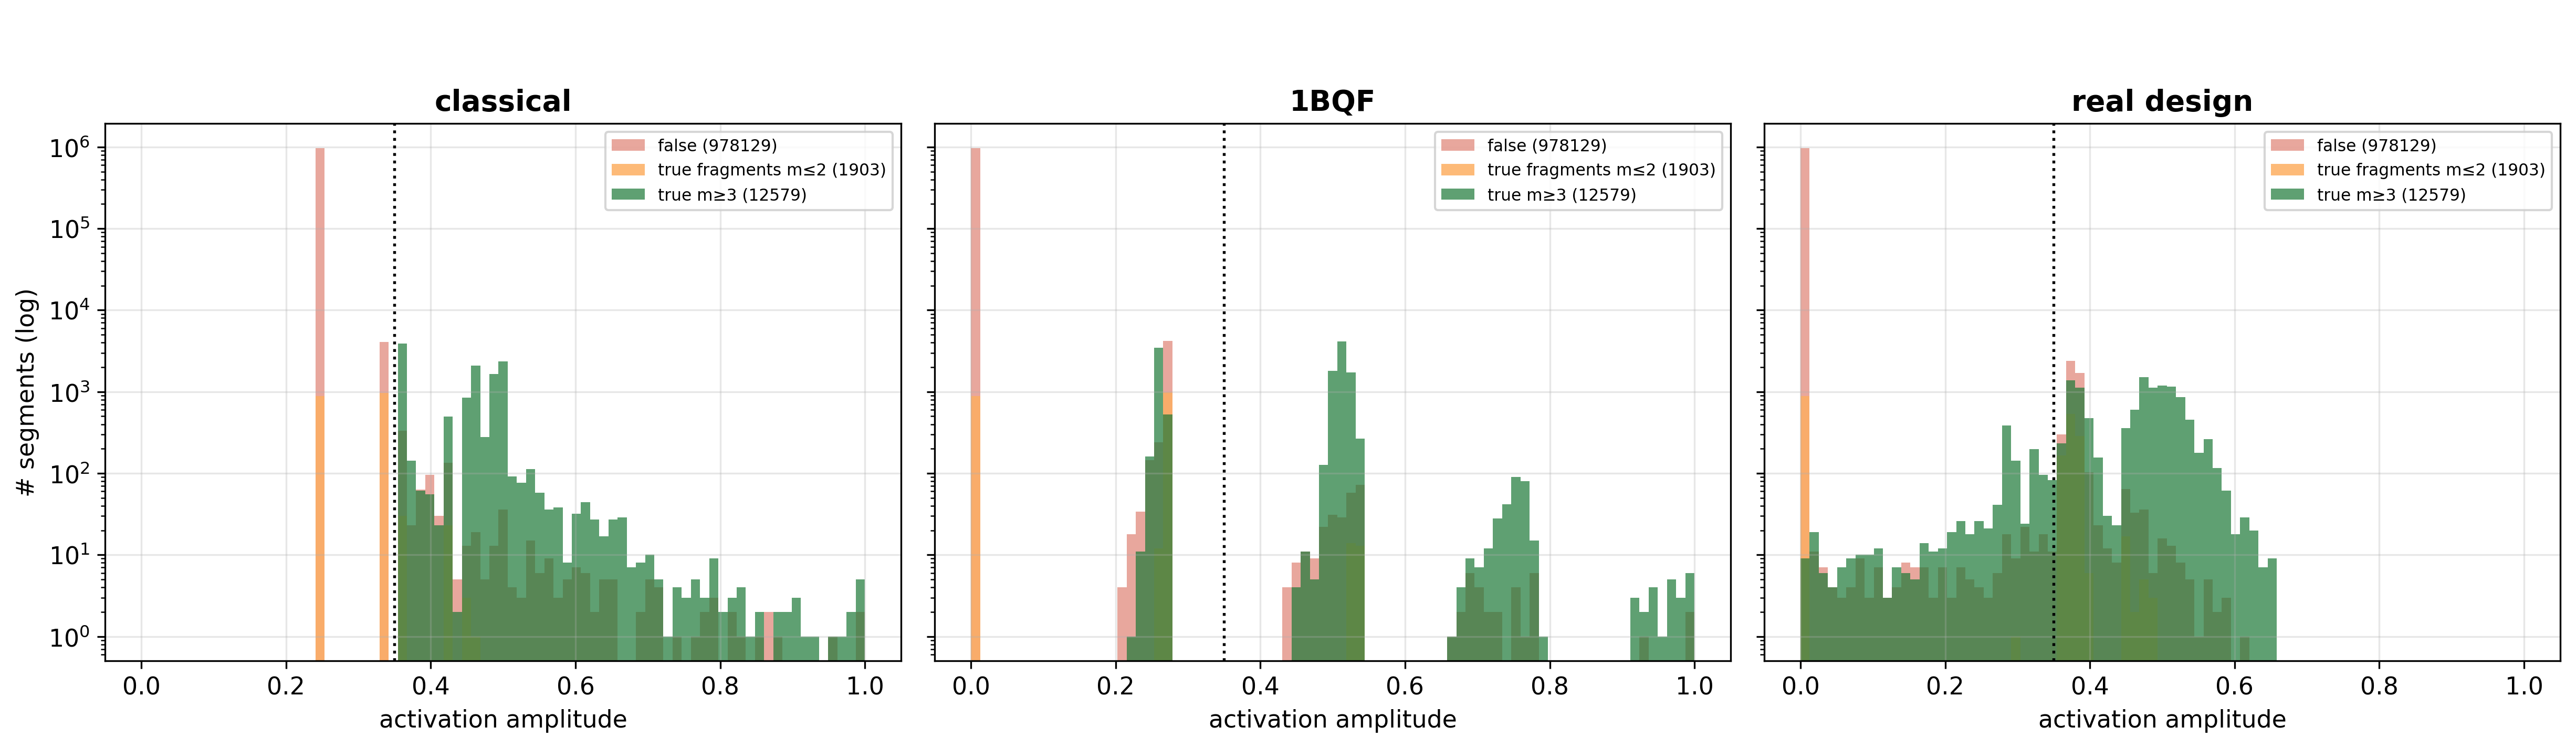
\includegraphics[width=0.98\textwidth]{run3_activation_spectra.png}
\caption{The real-geometry counterpart of the toy's amplitude
pile-up: activation-amplitude spectra on real Run-3 VELO event
geometry, for the classical solver, the 1BQF, and the redesigned
band-plus-notch response. Pink: false segments; orange: true
fragments ($m\le2$); green: findable true segments ($m\ge3$); the
dotted line is the fixed threshold. Variable track length smears
the discrete toy levels into bands, and the fragment population
sits inside the false bulk for every solver --- the real-geometry
form of the fragment floor.}
\label{fig:run3}
\end{figure}

% ══════════════════════════════════════════════════════════════════════════════
\section{Conclusion}
\label{sec:conclusion}

This paper set out to finish a thought that the one-bit quantum
filter started. The 1BQF's insight was that track finding does not
need a linear-system solution, only a spectral separation, and that
one cosine with one zero buys the largest separation in the problem
at almost no quantum cost. Promoting that cosine to the full QSVT
polynomial family converts algorithm design into response design,
and response design turns out to be a measurement-driven loop:

\begin{enumerate}[leftmargin=2em]
\item Read the spectrum the problem gives you. On clean events the
detector geometry hands you four exact eigenvalue lines, and a fixed
forty-degree comb pinned to them converts the segment selection at
$T=1000$ tracks from a $20.5\%$ false rate (the classical solver at
its fixed threshold) to $0.9\%$ (the comb at the same threshold, at
$92\%$ segment efficiency): a factor twenty fewer fakes in the
selected sample.
\item When the problem changes, measure where the false weight went,
and put roots there. At the heavy-noise operating point
($\sigma_{\rm res}=20\,\mu$m, $1\%$ hit drop, $T=200$) the false
weight piles up on the pair and triple motif lines, and the response
refitted to that measurement reads a false rate of $0.061$ at
matched segment efficiency $0.97$ where the classical solver on the
same events reads $0.124$ --- half the fakes at identical
efficiency, on every event tested, at every efficiency below the
fragment floor.
\item Judge every Hamiltonian modification together with the
response fitted to it, never separately. Both Denby--Peterson terms
destroy the degree-one filter, and both help the refitted
polynomial: the fork system fits to $0.046$ at matched efficiency
$0.97$ (against $0.061$ without the fork), and the occupancy system
at small coupling $\alpha=0.05$ fits to $0.039$ --- the best number
in the study, produced by the same term whose coupling collapses
the 1BQF's separation (AUC $0.996\to0.634$). Operator and response
are one design, not two.
\item Know what the spectrum cannot see --- and know that the
operator can change what that is. Spectral twins bound every
function of $\lambda$ on a fixed Hamiltonian, classical scoring
included; at heavy noise the true fragments of broken tracks are
twins of the false pairs, and on the base and fork systems they
floor every solver at segment efficiency $\approx0.98$: pushing to
$0.99$ floods the selection back to a $\approx0.65$ false rate for
everything. But the floor is a degeneracy of the operator, not of
the event: the occupancy coupling embeds each motif in its
hit-sharing neighbourhood, breaks the twin isomorphism, and the one
event that was floor-bound at $0.654$ on the base system fits to
$0.062$ on the occupancy system at the same matched efficiency.
\end{enumerate}

The open problems are, I think, unusually crisp for this field: a
single fixed response for the whole event ensemble --- on this toy
an enumeration over the finite motif structure (roots on the motif
lines, passes wide enough for the contaminated spread) rather than
a fitting problem, with the floor-breaking occupancy system folded
in; per-cluster realization as the structural
alternative to global filtering; edge-coloured synthesis for
weighted couplings on hardware; and the transplant of the whole
loop onto real detector geometry, where the structure is no longer
enumerable by hand, the response question needs closer thought, and
the first measurements say the method survives even though the comb
does not. Every cloud has
a silver lining: the same noise that broke the clean-event comb
handed us a false population parked on nameable eigenvalue lines,
and a filter family with exactly enough roots to meet it.

\section*{Acknowledgements}
To be completed 

% ══════════════════════════════════════════════════════════════════════════════
\begin{thebibliography}{99}

\bibitem{nicotra2023}
D.~Nicotra et al.,
\emph{A quantum algorithm for track reconstruction in the LHCb vertex
detector}, JINST \textbf{18} (2023) P11028.

\bibitem{hhl2009}
A.~W.~Harrow, A.~Hassidim and S.~Lloyd,
\emph{Quantum algorithm for linear systems of equations},
Phys.\ Rev.\ Lett.\ \textbf{103} (2009) 150502.

\bibitem{trackhhl}
X.~Chiotopoulos, D.~Nicotra, G.~Scriven, K.~Driessens, M.~Merk,
J.~Sch\"utz, J.~de~Vries and M.~H.~M.~Winands,
\emph{TrackHHL: The 1-Bit Quantum Filter for particle trajectory
reconstruction}, arXiv:2601.07766.

\bibitem{trackhhl_epj}
X.~Chiotopoulos, M.~L.~Martinez, D.~Nicotra, J.~A.~de~Vries,
K.~Driessens, M.~Merk and M.~H.~Winands,
\emph{TrackHHL: A Quantum Computing Algorithm for Track Reconstruction
at the LHCb}, EPJ Web Conf.\ \textbf{337} (2025) 01181;
arXiv:2511.11458.

\bibitem{denby1988}
B.~Denby,
\emph{Neural networks and cellular automata in experimental high
energy physics}, Comput.\ Phys.\ Commun.\ \textbf{49} (1988) 429.

\bibitem{peterson1989}
C.~Peterson,
\emph{Track finding with neural networks},
Nucl.\ Instrum.\ Meth.\ A \textbf{279} (1989) 537.

\bibitem{gslw2019}
A.~Gily\'en, Y.~Su, G.~H.~Low and N.~Wiebe,
\emph{Quantum singular value transformation and beyond: exponential
improvements for quantum matrix arithmetics},
Proc.\ 51st ACM STOC (2019) 193; arXiv:1806.01838.

\bibitem{lowchuang2019}
G.~H.~Low and I.~L.~Chuang,
\emph{Hamiltonian simulation by qubitization},
Quantum \textbf{3} (2019) 163.

\bibitem{childs2012}
A.~M.~Childs and N.~Wiebe,
\emph{Hamiltonian simulation using linear combinations of unitary
operations}, Quantum Inf.\ Comput.\ \textbf{12} (2012) 901.

\bibitem{martyn2021}
J.~M.~Martyn, Z.~M.~Rossi, A.~K.~Tan and I.~L.~Chuang,
\emph{Grand unification of quantum algorithms},
PRX Quantum \textbf{2} (2021) 040203.

\end{thebibliography}

\end{document}
